\documentclass[a4paper,12pt]{article}
\usepackage[utf8]{inputenc}
\usepackage[T1]{fontenc}
\usepackage[english]{babel}
% lmodern nicht verfügbar
\usepackage{amsmath}
\usepackage{amssymb}
\usepackage{amsthm}
\usepackage{geometry}
\usepackage{graphicx}
\usepackage[hidelinks]{hyperref}
\usepackage{listings}
\usepackage{xcolor}
\usepackage{enumitem}
\usepackage{booktabs}
\usepackage{caption}
\usepackage{subcaption}
\usepackage{float}
% microtype entfällt
\emergencystretch=4em

\geometry{margin=2.5cm}

\theoremstyle{definition}
\newtheorem{definition}{Definition}
\newtheorem{beispiel}{Beispiel}
\newtheorem{satz}{Satz}
\newtheorem{lemma}{Lemma}
\newtheorem{bemerkung}{Bemerkung}

\setlist[itemize,1]{label=--}

% Pfade zu den Ergebnissen des Experiment-Frameworks
\graphicspath{{../src/results/paper/}{../src/results/}}
\newcommand{\resultsdir}{../src/results}

% ---------- Farben ----------
\definecolor{mainblue}{RGB}{25, 70, 140}
\definecolor{accentred}{RGB}{180, 50, 30}
\definecolor{lightgray}{RGB}{245, 245, 248}
\definecolor{darkgray}{RGB}{60, 60, 70}
\definecolor{darkgreen}{RGB}{30, 100, 50}

\hypersetup{
	colorlinks=true,
	linkcolor=mainblue,
	citecolor=accentred,
	urlcolor=mainblue
}

%  Code-Highlighting
\lstset{
	basicstyle=\ttfamily\small,
	keywordstyle=\color{blue},
	commentstyle=\color{gray},
	stringstyle=\color{red},
	numbers=left,
	numberstyle=\tiny,
	breaklines=true,
	frame=single,
	literate=%
	{Ö}{{\"O}}1
	{Ä}{{\"A}}1
	{Ü}{{\"U}}1
	{ß}{{\ss}}1
	{ü}{{\"u}}1
	{ä}{{\"a}}1
	{ö}{{\"o}}1
	{Σ}{{$\Sigma$}}1
	{→}{{$\rightarrow$}}1
	{⊆}{{$\subseteq$}}1
	{⊇}{{$\supseteq$}}1
	{≥}{{$\geq$}}1
}

\captionsetup{font=small,labelfont=bf}
% ---------- Deutsche Bezeichnungen (Ersatz für babel-german) ----------
\addto\captionsenglish{%
  \renewcommand{\contentsname}{Inhaltsverzeichnis}%
  \renewcommand{\figurename}{Abbildung}%
  \renewcommand{\tablename}{Tabelle}%
  \renewcommand{\abstractname}{Kurzfassung}%
  \renewcommand{\refname}{Literatur}%
  \renewcommand{\appendixname}{Anhang}%
  \renewcommand{\listfigurename}{Abbildungsverzeichnis}%
  \renewcommand{\listtablename}{Tabellenverzeichnis}%
  \renewcommand{\proofname}{Beweis}%
  \renewcommand{\lstlistingname}{Listing}%
}
\renewcommand{\sectionautorefname}{Abschnitt}
\renewcommand{\subsectionautorefname}{Abschnitt}
\renewcommand{\figureautorefname}{Abbildung}
\renewcommand{\tableautorefname}{Tabelle}
\def\monthname{}
\makeatletter
\def\today{\number\day.~\ifcase\month\or Januar\or Februar\or M\"arz\or April\or Mai\or Juni\or Juli\or August\or September\or Oktober\or November\or Dezember\fi\space\number\year}
\makeatother


\title{Experimentelle Analyse\\Subgraph-SAT-Solver auf Boolean Circuits}
\author{\textsc{Stephan Epp}\\ {\small \texttt{\textbf{M.Sc.}}}}
\date{10. Oktober 2026}

\begin{document}

\maketitle

\begin{abstract}
\noindent
Wir berichten über 288 Benchmark-Läufe des Subgraph-SAT-Solvers auf drei Familien von Boolean Circuits: synthetischen Target-AND-Circuits (4 bis 20 Eingänge), Target-AND-Circuits mit zufälligen Zwischenschichten (Tiefe 1 bis 12) und den zwölf ISCAS'85-Benchmarks mit bis zu 3\,512 Gates und 10\,690 CNF-Klauseln. Die Läufe verteilen sich auf vier Experiment-Suites (Quick, Standard, Full, Performance). Die gemessenen Laufzeiten liegen zwischen 6,02 und 40,27\,ms (Mittelwert 21,81\,ms, Standardabweichung 7,25\,ms). Sie zeigen \emph{keinen} statistisch nachweisbaren Zusammenhang mit Gate-Anzahl, Klauselzahl, Eingangszahl oder Tiefe ($|\rho| \le 0{,}11$, alle $p > 0{,}1$) und unterscheiden sich weder zwischen den Circuit-Typen noch zwischen den Suites signifikant. Rund 60\,\% der Messwerte liegen innerhalb von $\pm 1$\,ms um das Einfache oder Doppelte von 15,625\,ms, der typischen Auflösung der verwendeten Wallclock-Messung. Wir schließen daraus, dass die Messungen durch Prozessstart und Zeitauflösung dominiert werden und nur eine \emph{obere Schranke} der Solver-Laufzeit liefern, jedoch keine Aussage über das Skalierungsverhalten des Algorithmus erlauben. Zusätzlich dokumentieren wir, dass in allen Läufen weder eine Solver-Ausgabe noch ein Erfüllbarkeitsergebnis erfasst wurde und dass der CNF-Encoder die Gate-Typen NAND, NOR und XOR fehlerhaft kodiert. Wir leiten daraus konkrete Verbesserungen des Messaufbaus ab.
\end{abstract}

\tableofcontents
\newpage

%=====================================================================
\section{Einführung}

Der Subgraph Algorithmus~\cite{epp-subgraph} vergleicht zwei Graphen anhand von Adjazenzmatrizen und Signatur-Arrays und besitzt eine Laufzeit von $O(n^3)$. Der Subgraph-SAT-Solver überträgt diese Idee auf das Erfüllbarkeitsproblem aussagenlogischer Formeln in konjunktiver Normalform (CNF). Die hier verwendeten Target-AND-Circuits und die zugehörigen Experimentreihen gehen auf die Masterarbeit des Autors~\cite{epp2013} zurück. Das vorliegende Projekt \texttt{subgraph-sat-solver-experiments} ist ein Python-Framework, das Boolean Circuits erzeugt, sie in das DIMACS-CNF-Format übersetzt, den Solver als externen Prozess aufruft, die Laufzeit misst und die Ergebnisse als JSON, CSV und Diagramme ablegt.

Diese Arbeit führt alle bisher erzeugten Ergebnisse dieses Frameworks zusammen und wertet sie statistisch aus.

\subsection{Fragestellungen}

Die Experimente sollten folgende Fragen beantworten:
\begin{enumerate}[label=\textbf{F\arabic*}]
	\item Wie verhält sich die Laufzeit des Solvers bei wachsender Anzahl der Eingänge $m$ (Target-AND-Circuits)?
	\item Wie verhält sich die Laufzeit bei wachsender Tiefe $d$ zufälliger Zwischenschichten (Target-AND-Random)?
	\item Wie verhält sich der Solver auf industriellen Standard-Benchmarks (ISCAS'85)?
	\item Wie reproduzierbar sind die Messungen über verschiedene Suites hinweg?
\end{enumerate}

\subsection{Beitrag}

\begin{itemize}
	\item Vollständige Darstellung des Experimentaufbaus und aller 288 Messwerte (Abschnitte~\ref{sec:aufbau} und~\ref{sec:ergebnisse}).
	\item Eine statistische Auswertung (Korrelationen, Rangtests), die zeigt, dass die Laufzeit in den vorliegenden Messungen unabhängig von der Instanzgröße ist.
	\item Eine kritische Einordnung der Messmethodik: Zeitauflösung, fehlende Solver-Ausgabe und Kodierung (Abschnitt~\ref{sec:diskussion}).
	\item Ein reproduzierbares Auswertungsskript (\texttt{src/paper\_analysis.py}), das alle Tabellen und Abbildungen dieser Arbeit direkt aus den Rohdaten erzeugt (Anhang~\ref{sec:repro}).
\end{itemize}

%=====================================================================
\section{Grundlagen}

\subsection{Boolean Circuits und CNF}

\begin{definition}[Boolean Circuit]
	Ein Boolean Circuit mit $m$ Eingängen ist eine geordnete Liste von Gates $g_1, \ldots, g_k$. Jedes Gate hat einen Typ aus $\{\mathrm{NOT}, \mathrm{AND}, \mathrm{OR}, \mathrm{NAND}, \mathrm{NOR}, \mathrm{XOR}\}$ und bezieht seine Eingaben von Eingängen oder von früheren Gates. Die Größe des Circuits ist die Gate-Anzahl $k$.
\end{definition}

\begin{definition}[CNF]
	Eine Formel in konjunktiver Normalform (CNF) ist eine Konjunktion von Klauseln, wobei jede Klausel eine Disjunktion von Literalen ist. Das Erfüllbarkeitsproblem (SAT) fragt, ob eine Belegung der Variablen existiert, die alle Klauseln erfüllt~\cite{cook1971}.
\end{definition}

Die Übersetzung eines Circuits in CNF erfolgt mit der Tseitin-Transformation~\cite{tseitin1968}: Jedes Gate erhält eine eigene Variable $y$, und lokale Klauseln erzwingen $y \leftrightarrow \mathrm{op}(x_1, \ldots)$. Die Formelgröße wächst dadurch linear in der Gate-Anzahl.

\subsection{Implementierung des Subgraph-SAT-Solvers}
\label{sec:solver-impl}

Der untersuchte Solver ist ein in C++17 implementiertes Kommandozeilenprogramm und zugleich als statische Bibliothek nutzbar. Sein SAT-Verfahren besteht aus einer Reduktionspipeline und einem separaten Subgraph-Programm; der C++-Teil implementiert also nicht selbst den Subgraph Algorithmus. Abbildung und Phasenmessung lassen sich wie folgt zusammenfassen:

\begin{center}
\texttt{DIMACS-CNF $\rightarrow$ 3-SAT $\rightarrow$ Clique-Graph $\rightarrow$ Subgraph-Instanz $\rightarrow$ externes Programm}
\end{center}

\subsubsection{Einlesen und Normalisieren der Formel}

Die Kommandozeilenschnittstelle erwartet eine DIMACS-CNF-Datei. Alternativ kann die Bibliothek eine Formel als Zeichenkette oder als bereits geparstes Objekt entgegennehmen. Literale werden intern als vorzeichenbehaftete ganze Zahlen dargestellt: Eine positive Zahl bezeichnet eine Variable, eine negative deren Negation. Vor der Graphkonstruktion kopiert der Reduktor die Formel und wandelt Klauseln mit mehr als drei Literalen durch zusätzliche Hilfsvariablen in Klauseln mit höchstens drei Literalen um. Klauseln mit höchstens drei Literalen bleiben unverändert. Anschließend entfernt \texttt{simplify()} doppelte Klauseln und Tautologien; die separat vorhandene Unit-Propagation-Routine wird in diesem Ausführungspfad nicht aufgerufen. Die Reduktion verändert damit eine interne Kopie, während die ursprüngliche Formel für die spätere Ergebnisvalidierung erhalten bleibt.

\subsubsection{Reduktion von 3-SAT auf Clique}

Für jedes Literalvorkommen wird ein eigener Knoten angelegt. Ein Knoten speichert dabei implizit, aus welcher Klausel und an welcher Position das Literal steht. Zwei Knoten werden genau dann durch eine ungerichtete Kante verbunden, wenn sie aus verschiedenen Klauseln stammen und ihre Literale nicht unmittelbar im Widerspruch stehen. Für die Literale $x_i$ und $x_j$ bedeutet das insbesondere, dass zwischen einem Vorkommen von $x$ und einem Vorkommen von $\neg x$ keine Kante liegt. Zwischen zwei Knoten derselben Klausel gibt es ebenfalls keine Kante.

Gesucht wird eine Clique der Größe $k$, wobei $k$ der Anzahl der Klauseln der normalisierten Formel entspricht. Eine erfüllende Belegung liefert eine solche Clique, indem aus jeder Klausel ein unter dieser Belegung wahres Literal ausgewählt wird: Die ausgewählten Knoten stammen aus verschiedenen Klauseln und widersprechen einander nicht. Umgekehrt enthält eine Clique der Größe $k$ wegen der fehlenden Kanten innerhalb einer Klausel genau einen Knoten je Klausel; wegen der fehlenden Kanten zwischen komplementären Literalen sind die gewählten Literale miteinander verträglich. Sie können daher gemeinsam wahr gesetzt werden und erfüllen jede Klausel. Dies ist die intendierte Korrektheitsbeziehung der Reduktion.

Der Clique-Graph wird durch eine boolesche Adjazenzmatrix repräsentiert. Bezeichnet $L$ die Zahl der Literalvorkommen nach der Normalisierung, besitzt der Graph $L$ Knoten; die Kanten werden durch paarweisen Vergleich der Knoten konstruiert. Die Konstruktion benötigt damit $O(L^2)$ Paarprüfungen und die Matrix $O(L^2)$ Speicherplätze. Der Code prüft vor dieser Stufe, dass keine Klausel mehr als drei Literale enthält.

Listing~\ref{lst:clique-reduction} zeigt den Kern dieser Konstruktion in C++17. Für jedes Literalvorkommen wird ein Knoten angelegt; die Adjazenzmatrix erhält genau dann eine Kante, wenn zwei Knoten aus verschiedenen Klauseln stammen und ihre Literale nicht komplementär sind. Der Rückgabewert enthält außerdem die gesuchte Clique-Größe $k$, die der Anzahl der Klauseln entspricht. Das Beispiel erläutert die Reduktionsidee und ist kein wörtlicher Auszug aus dem Solver-Quelltext.

\begin{lstlisting}[language=C++, caption={Didaktischer C++17-Auszug: Konstruktion der Clique-Instanz aus einer 3-CNF-Formel}, label={lst:clique-reduction}]
#include <cstddef>
#include <stdexcept>
#include <utility>
#include <vector>

struct CliqueInstance {
    std::vector<std::vector<bool>> adjacency;
    std::size_t targetSize;
};

struct LiteralNode {
    std::size_t clause;
    int literal;
};

CliqueInstance makeCliqueInstance(
    const std::vector<std::vector<int>>& clauses) {
    std::vector<LiteralNode> nodes;
    for (std::size_t c = 0; c < clauses.size(); ++c) {
        if (clauses[c].size() > 3) {
            throw std::invalid_argument("formula is not 3-CNF");
        }
        for (int literal : clauses[c]) {
            nodes.push_back({c, literal});
        }
    }

    std::vector<std::vector<bool>> adjacency(
        nodes.size(), std::vector<bool>(nodes.size(), false));
    for (std::size_t i = 0; i < nodes.size(); ++i) {
        for (std::size_t j = i + 1; j < nodes.size(); ++j) {
            const auto& a = nodes[i];
            const auto& b = nodes[j];
            const bool differentClauses = a.clause != b.clause;
            const bool complementary = a.literal == -b.literal;
            if (differentClauses && !complementary) {
                adjacency[i][j] = true;
                adjacency[j][i] = true;
            }
        }
    }
    return {std::move(adjacency), clauses.size()};
}
\end{lstlisting}

\subsubsection{Reduktion von Clique auf Subgraph-Isomorphismus}

Der Clique-Graph wird zum Quellgraphen $G$. Als Zielgraph $H$ wird der vollständige Graph $K_k$ mit $k$ Knoten erzeugt. Da jede Kante von $K_k$ im Quellgraphen vorhanden sein muss, ist $K_k$ genau dann ein Teilgraph von $G$, wenn $G$ eine Clique der Größe $k$ enthält. Beide Graphen werden mit Knotenbezeichnern wie \texttt{v0} und einer Kantenliste in JSON serialisiert. Die äußere JSON-Struktur enthält die Schlüssel \texttt{G} und \texttt{H}.

Der Solver schreibt diese Daten in temporäre Dateien und startet das konfigurierte Subgraph-Binary als separaten Prozess. Unter Windows geschieht dies über \texttt{system()}, unter Unix-artigen Systemen über \texttt{fork()} und \texttt{execl()}. Das externe Programm muss die Eingabe- und Ausgabedatei als Kommandozeilenargumente akzeptieren. Damit hängt die praktische Entscheidung nicht nur von der Reduktionsimplementierung, sondern auch von einem kompatiblen externen Binary samt JSON-Schnittstelle ab.

\subsubsection{Ergebnisverarbeitung und Belegung}

Die Ausgabedatei des Subgraph-Programms wird nicht als JSON geparst. Stattdessen sucht der Solver nach der exakten Zeichenfolge \texttt{"is\_subgraph": true}. Wird sie gefunden, gilt die Subgraph-Instanz als positiv; andernfalls wird sie als negativ und damit die SAT-Formel als unerfüllbar eingestuft. Ein Prozessfehler führt zu \texttt{SAT\_ERROR}. Die Konfiguration enthält zwar ein Zeitlimit, der Prozessaufruf setzt dieses in der vorliegenden Implementierung jedoch nicht durch.

Für eine vollständige SAT-Lösung müsste das vom Subgraph-Programm gefundene Knotenmapping zurückgegeben und auf die ausgewählten Literalvorkommen abgebildet werden. Dieser Schritt fehlt im aktuellen Aufrufpfad: Das Mapping wird weder aus der Ausgabe gelesen noch an den vorhandenen Extraktor übergeben. Bei positivem Subgraph-Ergebnis setzt der Solver stattdessen jede Variable der ursprünglichen Formel auf wahr. Die standardmäßig aktive Validierung prüft diese Belegung gegen die ursprüngliche CNF; schlägt sie fehl, lautet das Ergebnis \texttt{SAT\_ERROR}. Ein positives Subgraph-Ergebnis allein garantiert daher in dieser Implementierung noch keine zurückgegebene, gültige SAT-Belegung.

\subsubsection{Laufzeitmessung und Einordnung}

Der Ergebnistyp erfasst getrennte Zeiten für Reduktion, Aufruf des Subgraph-Prozesses und Extraktion sowie eine Gesamtzeit. Die Zeit des Prozessaufrufs umfasst dabei auch die zugehörige Datei-I/O und den Prozessstart; sie ist keine isolierte Messung der Rechenzeit des externen Algorithmus. Die Reduktionsstufe baut zunächst einen Graphen auf, dessen Größe quadratisch mit der Zahl der Literalvorkommen wachsen kann. Die in der theoretischen Grundlage angegebene Schranke $\Theta(n^3)$ bezieht sich auf den Subgraph Algorithmus~\cite{epp-subgraph}; sie beschreibt weder automatisch die Kosten der gesamten Implementierung noch belegt sie deren Korrektheit. Ob und wie sich diese Schranke im gemessenen Prozess auswirkt, ist nicht Gegenstand der Experimente (Abschnitt~\ref{sec:diskussion}).

Im Experiment-Framework wird das kompilierte Programm als Black Box aufgerufen: Das Framework erzeugt die Eingabe-CNF, startet den Prozess und misst die Wallclock-Zeit bis zu dessen Ende (Abschnitt~\ref{sec:messung}). Diese Messung ist von den internen Phasenzeiten der Solver-Bibliothek zu unterscheiden. Außerdem dokumentieren die Experimente, dass bei keinem der 288 Läufe ein SAT-Ergebnis erfasst wurde; somit weisen die Messdaten nicht nach, dass die beschriebene Pipeline in diesen Läufen eine gültige Lösung geliefert hat.

%=====================================================================
\section{Experimenteller Aufbau}
\label{sec:aufbau}

\subsection{Circuit-Familien}

\subsubsection{Target-AND}

Ein Target-AND-Circuit mit $m$ Eingängen $x_0, \ldots, x_{m-1}$ ist so konstruiert, dass sein Ausgang nur unter genau einer Eingabebelegung $a^*$ wahr wird. Diese Belegung wird durch die Halbierungsstrategie des LBV-Verfahrens (vgl.~\cite{epp2013}) bestimmt: Ausgehend von der Nullbelegung werden in jeder Runde die ersten $\lfloor m/2^r \rfloor$ Eingänge invertiert, $r = 1, 2, \ldots$, bis die Blockgröße $0$ erreicht. Der Circuit besteht aus je einem NOT-Gate pro Eingang und einem balancierten Binärbaum aus AND-Gates über die Literale von $a^*$.

\begin{satz}[Größe der Target-AND-Circuits]
	\label{satz:groesse}
	Ein Target-AND-Circuit mit $m \ge 2$ Eingängen besitzt genau $2m-1$ Gates und seine Tseitin-CNF genau $6m-4$ Klauseln.
\end{satz}

\begin{proof}
	Es gibt $m$ NOT-Gates. Ein Binärbaum mit $m$ Blättern hat unabhängig von $m$ genau $m-1$ innere Knoten; jeder ist ein AND-Gate. Das ergibt $m + (m-1) = 2m-1$ Gates. Ein NOT-Gate erzeugt zwei Klauseln, ein AND-Gate mit zwei Eingängen vier (siehe Abschnitt~\ref{sec:cnf}). Insgesamt ergeben sich $2m + 4(m-1) = 6m-4$ Klauseln.
\end{proof}

Die Messdaten bestätigen dies für alle $m \in \{4, 6, \ldots, 20\}$ (Tabelle~\ref{tab:target_and}); beispielsweise besitzt $m=20$ genau $39$ Gates und $116$ Klauseln. Die Anzahl der LBV-Runden, die im Datensatz als Feld \texttt{lbv\_rounds} gespeichert ist, beträgt $\lfloor \log_2 m \rfloor + 1$ (3 Runden für $m \in \{4,6\}$, 4 für $m \in \{8,\ldots,14\}$, 5 für $m \in \{16,18,20\}$).

\subsubsection{Target-AND-Random}

Dieser Typ erweitert den Target-AND-Circuit mit $m=10$ Eingängen um $d \in \{1, \ldots, 12\}$ zufällige Zwischenschichten. Jede Schicht enthält $\max(2, \lfloor |L|/2 \rfloor + r)$ Gates mit $r \in \{0,1,2\}$ gleichverteilt, wobei $|L|$ die Größe der vorherigen Schicht ist. Jedes Gate hat einen zufälligen Typ aus $\{\mathrm{AND}, \mathrm{OR}, \mathrm{NAND}, \mathrm{NOR}, \mathrm{XOR}\}$ und zwei oder drei zufällig gewählte Eingänge der vorherigen Schicht. Ein abschließendes AND-Gate verknüpft das Target-AND mit dem ersten Gate der letzten Zufallsschicht. Der Zufallsgenerator wird in jedem Circuit mit dem festen Seed $42$ initialisiert, sodass die Circuits deterministisch sind und der Circuit der Tiefe $d+1$ den Circuit der Tiefe $d$ (bis auf das abschließende AND-Gate) um eine weitere Schicht ergänzt.

\subsubsection{ISCAS'85}

Die ISCAS'85-Benchmarks~\cite{brglez1985} sind kombinatorische Standard-Schaltkreise aus der Hardware-Verifikation. Das Framework liest die \texttt{.bench}-Dateien aus \texttt{src/iscas85/} ein. Es werden die zehn klassischen Circuits c432 bis c7552 sowie zwei kleine Beispielcircuits (c3 mit 4 und c17 mit 6 Gates) verwendet. Zwei Circuits sind funktional verwandt: c1355 ist die Variante von c499, in der die XOR-Gates durch NAND-Gates ersetzt wurden.

\subsection{CNF-Kodierung}
\label{sec:cnf}

Für ein Gate mit Variable $y$ und Eingangsvariablen $x_1, \ldots, x_k$ erzeugt das Framework folgende Klauseln:

\begin{center}
\begin{tabular}{lll}
\toprule
Gate & Klauseln & Anzahl \\
\midrule
NOT & $(\neg y \vee \neg x_1),\ (y \vee x_1)$ & 2 \\
AND & $(\neg y \vee x_1 \vee \ldots \vee x_k),\ (\neg y \vee x_i)_{i},\ (y \vee \neg x_1 \vee \ldots \vee \neg x_k)$ & $k+2$ \\
OR & $(y \vee \neg x_1 \vee \ldots \vee \neg x_k),\ (y \vee \neg x_i)_{i},\ (\neg y \vee x_1 \vee \ldots \vee x_k)$ & $k+2$ \\
NAND, NOR & Klauselmuster von OR bzw.\ AND (siehe unten) & $k+2$ \\
XOR & vier Klauseln über $y, x_1, x_2$ (siehe unten) & 4 \\
\bottomrule
\end{tabular}
\end{center}

Eine Überprüfung der Kodierung für jedes Gate-Muster mit allen Eingabe\-kombinationen ergibt, dass AND, OR und NOT korrekt kodiert sind, NAND, NOR und XOR jedoch nicht: Im Quelltext verwendet NAND dasselbe Klauselmuster wie OR, NOR dasselbe wie AND, und die vier XOR-Klauseln beschreiben $y \leftrightarrow \neg(x_1 \oplus x_2)$ (XNOR). Damit beschreiben die erzeugten CNF-Dateien für Gates dieser drei Typen nicht die Funktion des ursprünglichen Circuits. Das betrifft vor allem ISCAS'85, dessen Circuits überwiegend aus NAND-, NOR- und XOR-Gates bestehen (c17 enthält ausschließlich NAND-Gates, c6288 besteht zu etwa $88\,\%$ aus NAND-, NOR- und XOR-Gates), sowie die zufälligen Zwischenschichten von Target-AND-Random. Die Target-AND-Circuits verwenden nur NOT und AND und sind nicht betroffen. Wir haben die Kodierung für diese Arbeit nicht verändert, damit die dokumentierten Ergebnisse den tatsächlich ausgeführten Experimenten entsprechen.

Die Kodierung enthält \emph{keine} Unit-Klausel, die den Ausgang des Circuits auf wahr festlegt. Jede Eingabebelegung lässt sich daher zu einer erfüllenden Belegung der Gesamtformel fortsetzen, die erzeugten Formeln sind unabhängig vom Circuit erfüllbar. Auf diesen Punkt kommen wir in Abschnitt~\ref{sec:diskussion} zurück.

\subsection{Messmethodik}
\label{sec:messung}

Jeder Lauf schreibt die CNF in eine temporäre Datei und startet den Solver per \texttt{subprocess.run} mit einem Timeout von 30\,s. Gemessen wird die Wallclock-Zeit $t$ zwischen \texttt{time.time()} vor dem Start und nach dem Ende des Prozesses, in Millisekunden. Die gemessene Zeit umfasst damit Prozessstart, Einlesen der Datei, Lösen und Prozessende. Als erfüllbar gilt eine Instanz, wenn die Zeichenkette \texttt{SAT} in Standardausgabe oder Fehlerausgabe vorkommt und \texttt{UNSAT} nicht. Der Speicherverbrauch wird nicht erfasst (das Feld \texttt{memory\_usage\_mb} ist stets $0$). Pro Lauf werden Circuit-Typ, Name, Anzahl Eingänge, Gates und Klauseln, Erfüllbarkeit, Laufzeit, Zeitstempel, LBV-Runden und Metadaten als JSON und CSV gespeichert.

\subsection{Experiment-Suites}

Die vier Suites unterscheiden sich in Umfang und Wiederholungszahl (Tabelle~\ref{tab:suites}). Quick und Standard enthalten jeden Circuit einmal, Full und Performance fünfmal (Target-AND und Target-AND-Random) bzw.\ einmal (ISCAS'85). Insgesamt entstehen $288$ Läufe: $108$ Target-AND, $144$ Target-AND-Random und $36$ ISCAS'85. Full und Performance sind in Umfang und Zusammensetzung identisch. Die Suites wurden am 14.\,Juli 2026 zwischen 09:40:03 und 09:40:48 Uhr ausgeführt.

\begin{table}[ht]
\centering\small
\setlength{\tabcolsep}{4pt}
\input{\resultsdir/paper/tab_suites.tex}
\caption{Die vier Experiment-Suites. T-AND: Target-AND, T-AND-R: Target-AND-Random. $\bar{t}$: Mittelwert, $s$: Standardabweichung, $\tilde{t}$: Median der Laufzeit. Die Dauer ist aus den Zeitstempeln (Auflösung 1\,s) als obere Schranke abgeleitet.}
\label{tab:suites}
\end{table}

\subsection{Statistische Auswertung}

Alle Kennzahlen werden aus den CSV-Dateien der Suites berechnet. Verwendet werden Mittelwert $\bar{t}$, Standardabweichung $s$ (mit $n-1$), Median, Quartile $Q_1, Q_3$, Minimum und Maximum. Zusammenhänge werden mit der Rangkorrelation nach Spearman ($\rho$) und der Pearson-Korrelation ($r$) sowie einer linearen Regression geprüft. Da die Laufzeiten deutlich nicht normalverteilt sind (Abbildung~\ref{fig:hist}), verwenden wir für Gruppenvergleiche rangbasierte Tests: Kruskal--Wallis für mehr als zwei Gruppen und Mann--Whitney-$U$ für zwei Gruppen. Das Signifikanzniveau beträgt $\alpha = 0{,}05$.

%=====================================================================
\section{Ergebnisse}
\label{sec:ergebnisse}

\subsection{Gesamtüberblick}

Über alle 288 Läufe liegt die Laufzeit zwischen $6{,}02$\,ms und $40{,}27$\,ms; der Mittelwert beträgt $21{,}81$\,ms, die Standardabweichung $7{,}25$\,ms und der Median $19{,}65$\,ms. Kein Lauf endete mit einem Fehler oder einem Timeout. Die Instanzen decken eine große Größenspanne ab (Tabelle~\ref{tab:structure}): von 4 bis 3\,512 Gates (Faktor 878) und von 14 bis 10\,690 Klauseln (Faktor 764).

\begin{table}[ht]
\centering\small
\input{\resultsdir/paper/tab_structure.tex}
\caption{Strukturelle Eigenschaften der Instanzen je Circuit-Typ (pro eindeutigem Circuit). $\bar{g}$: mittlere Gate-Anzahl, $\bar{k}$: mittlere Klauselzahl.}
\label{tab:structure}
\end{table}

Tabelle~\ref{tab:suite_type} zeigt die Laufzeitstatistik für jede Kombination aus Suite und Circuit-Typ. Die Mittelwerte liegen in allen elf Zellen zwischen $19{,}2$ und $25{,}7$\,ms, die Mediane zwischen $16{,}0$ und $28{,}3$\,ms.

\begin{table}[ht]
\centering\footnotesize
\setlength{\tabcolsep}{3.5pt}
\input{\resultsdir/paper/tab_suite_type.tex}
\caption{Laufzeitstatistik (in ms) je Suite und Circuit-Typ. Alle Werte stammen aus den \texttt{experiment\_results.csv}-Dateien der Suites.}
\label{tab:suite_type}
\end{table}

\begin{figure}[ht]
\centering
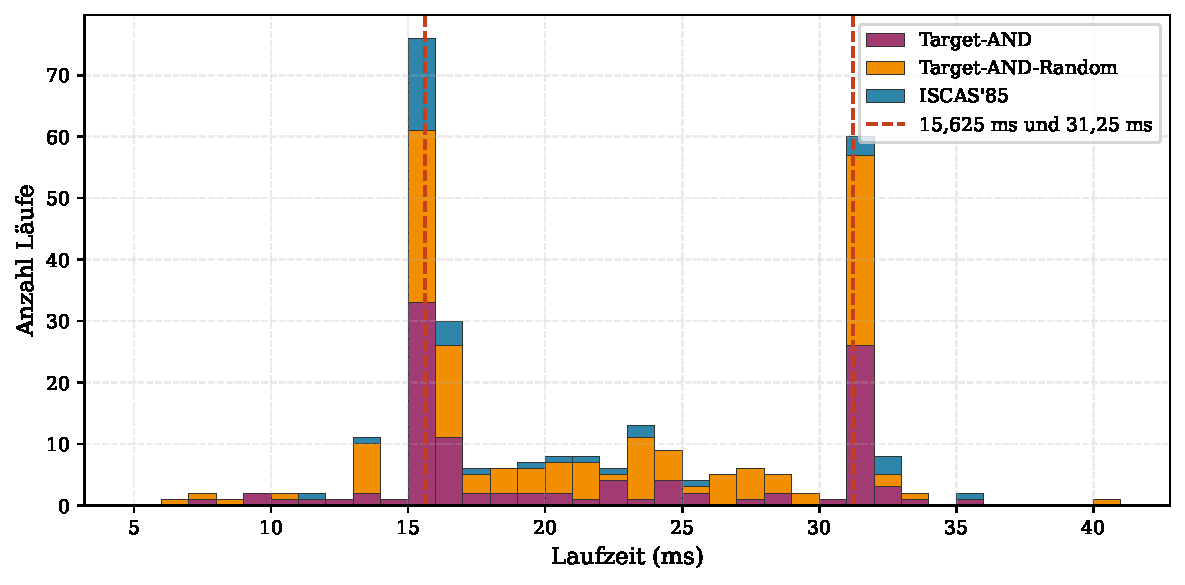
\includegraphics[width=0.92\textwidth]{fig_runtime_histogram.pdf}
\caption{Verteilung aller 288 Laufzeiten (Klassenbreite 1\,ms), gestapelt nach Circuit-Typ: Target-AND (violett), Target-AND-Random (orange), ISCAS\textquotesingle 85 (blau). Die roten gestrichelten Linien markieren $15{,}625$\,ms und $31{,}25$\,ms.}
\label{fig:hist}
\end{figure}

\paragraph{Aufbau der Abbildung.} Abbildung~\ref{fig:hist} ist ein gestapeltes Histogramm. Auf der Abszisse ist die gemessene Laufzeit in Millisekunden aufgetragen, unterteilt in Klassen der Breite $1$\,ms (von $5$ bis $41$\,ms); die Ordinate zählt die Läufe je Klasse. Jede Säule besteht aus bis zu drei übereinandergestapelten Farbsegmenten: Target-AND (violett, unten), Target-AND-Random (orange, Mitte) und ISCAS'85 (blau, oben). Die Gesamthöhe einer Säule ist die Anzahl aller Läufe in dieser Klasse, die Höhe eines Segments die Anzahl der Läufe des jeweiligen Typs. Die beiden roten, gestrichelten senkrechten Linien markieren $15{,}625$\,ms ($=1/64$\,s) und $31{,}25$\,ms ($=2/64$\,s); ihre Bedeutung wird in Abschnitt~\ref{sec:zeit} erläutert. Da die drei Typen mit $108$, $144$ und $36$ Läufen unterschiedlich stark vertreten sind, lassen sich die Segmenthöhen nicht unmittelbar als Anteile je Typ lesen.

\paragraph{Die beiden dominierenden Säulen.} Das Bild wird von zwei hohen, schmalen Säulen beherrscht, die jeweils unmittelbar auf einer der roten Linien stehen. Die Klasse $[15;16)$\,ms enthält $76$ Läufe ($26{,}4\,\%$ aller Läufe), nämlich $33$ Target-AND-, $28$ Target-AND-Random- und $15$ ISCAS-Läufe. Die Klasse $[31;32)$\,ms enthält $60$ Läufe ($20{,}8\,\%$), davon $26$, $31$ bzw.\ $3$. Diese beiden von insgesamt $36$ Klassen vereinen damit $136$ der $288$ Läufe ($47{,}2\,\%$). Rechts neben der ersten Säule schließt sich als Schulter die Klasse $[16;17)$\,ms mit $30$ Läufen an ($11$ Target-AND, $15$ Target-AND-Random, $4$ ISCAS), rechts neben der zweiten Säule die Klasse $[32;33)$\,ms mit $8$ Läufen. In beiden Säulen sind alle drei Farben vertreten; die Häufungen sind also nicht an einen einzelnen Circuit-Typ gebunden. Auffällig ist lediglich, dass ISCAS'85 mit $15$ von $36$ Läufen ($41{,}7\,\%$) in der unteren, aber nur mit $3$ von $36$ Läufen ($8{,}3\,\%$) in der oberen Säule steht. Bei $36$ Läufen und dem nicht signifikanten Mann--Whitney-Test zwischen ISCAS'85 und den synthetischen Circuits ($p = 0{,}140$, Tabelle~\ref{tab:tests}) lässt sich daraus jedoch keine Tendenz ableiten.

\paragraph{Der Bereich dazwischen und die Ränder.} Zwischen den beiden Säulen verläuft ein flacher Bereich: Die $14$ Klassen von $17$ bis $31$\,ms enthalten zusammen $86$ Läufe, im Mittel gut $6$ je Klasse. Die höchste dieser Klassen ist $[23;24)$\,ms mit $13$ Läufen; zu größeren Laufzeiten hin wird der Bereich dünner, bis die Klasse $[30;31)$\,ms nur noch einen einzigen Lauf enthält. In diesem Mittelbereich überwiegen die orangen Segmente: $54$ der $86$ Läufe stammen von Target-AND-Random, $24$ von Target-AND und $8$ von ISCAS'85. Am linken Rand liegen $23$ Läufe unterhalb von $15$\,ms, verteilt auf die Klassen von $6$ bis $14$\,ms. Dort fällt die Klasse $[13;14)$\,ms mit $11$ Läufen ($8$ Target-AND-Random, $2$ Target-AND, $1$ ISCAS) als kleine Nebenspitze auf; ihre Ursache lässt sich aus den Daten nicht bestimmen. Am rechten Rand liegen nur $5$ Läufe oberhalb von $33$\,ms ($33{,}70$, $33{,}83$, $35{,}24$, $35{,}50$ und $40{,}27$\,ms). Der Maximalwert von $40{,}27$\,ms ist ein einzelner Ausreißer (Target-AND-Random, $d=2$) in der sonst leeren Klasse $[40;41)$\,ms.

\paragraph{Interpretation.} Dass fast die Hälfte aller Läufe in zwei Klassen liegt, deren Mitten genau um einen Zeittakt von $15{,}625$\,ms auseinanderliegen, ist der zentrale Befund dieser Abbildung. Wäre die gemessene Zeit im Wesentlichen die Rechenzeit des Solvers, wäre für Instanzen von $4$ bis $3\,512$ Gates eine breite, mit der Größe verschobene Verteilung zu erwarten. Die beobachtete Form ist dagegen mit einer Messung vereinbar, deren Zeitauflösung grob ist (Abschnitt~\ref{sec:zeit}). Die Verteilung sollte daher nicht als Mischung aus \glqq schnellen\grqq{} und \glqq langsamen\grqq{} Instanzen gedeutet werden.

\subsection{Target-AND: Variation der Eingangszahl (F1)}

Tabelle~\ref{tab:target_and} fasst die Läufe nach Eingangszahl $m$ zusammen (je 12 Läufe über alle Suites). Gate- und Klauselzahl wachsen wie in Satz~\ref{satz:groesse} linear, von $7$ auf $39$ Gates. Die mittlere Laufzeit liegt für alle $m$ zwischen $17{,}49$\,ms ($m=4$) und $24{,}29$\,ms ($m=20$) und zeigt keinen Trend (Abbildung~\ref{fig:param}, links). Die Streuung innerhalb eines $m$-Wertes ($s = 6$ bis $8{,}6$\,ms) ist größer als der Unterschied der Mittelwerte zwischen verschiedenen $m$. Die Rangkorrelation zwischen Gate-Anzahl und Laufzeit beträgt $\rho = 0{,}106$ ($p = 0{,}275$, $n = 108$).

\begin{table}[ht]
\centering\small
\input{\resultsdir/paper/tab_target_and.tex}
\caption{Target-AND-Circuits: Struktur und Laufzeit (ms) je Eingangszahl $m$, über alle vier Suites aggregiert.}
\label{tab:target_and}
\end{table}

\subsection{Target-AND-Random: Variation der Tiefe (F2)}

Bei festem $m = 10$ wächst die Instanzgröße mit der Tiefe $d$ von $27$ Gates und $91$ Klauseln ($d=1$) auf $54$ Gates und $206$ Klauseln ($d=12$) (Tabelle~\ref{tab:depth}). Die mittlere Laufzeit schwankt unsystematisch zwischen $18{,}79$\,ms ($d=8$) und $26{,}57$\,ms ($d=5$); sie ist bei der größten Tiefe $d=12$ mit $20{,}56$\,ms kleiner als bei $d=1$ mit $23{,}08$\,ms. Die Rangkorrelation zwischen Tiefe und Laufzeit ist $\rho = -0{,}086$ ($p = 0{,}306$, $n = 144$). Die lineare Regression liefert eine Steigung von $-0{,}28$\,ms pro Tiefenschicht mit $R^2 = 0{,}018$. Ein tiefenabhängiger Anstieg ist damit nicht erkennbar (Abbildung~\ref{fig:param}, rechts).

\begin{table}[ht]
\centering\small
\input{\resultsdir/paper/tab_depth.tex}
\caption{Target-AND-Random-Circuits ($m=10$): Struktur und Laufzeit (ms) je Tiefe $d$, über alle vier Suites aggregiert.}
\label{tab:depth}
\end{table}

\begin{figure}[ht]
\centering
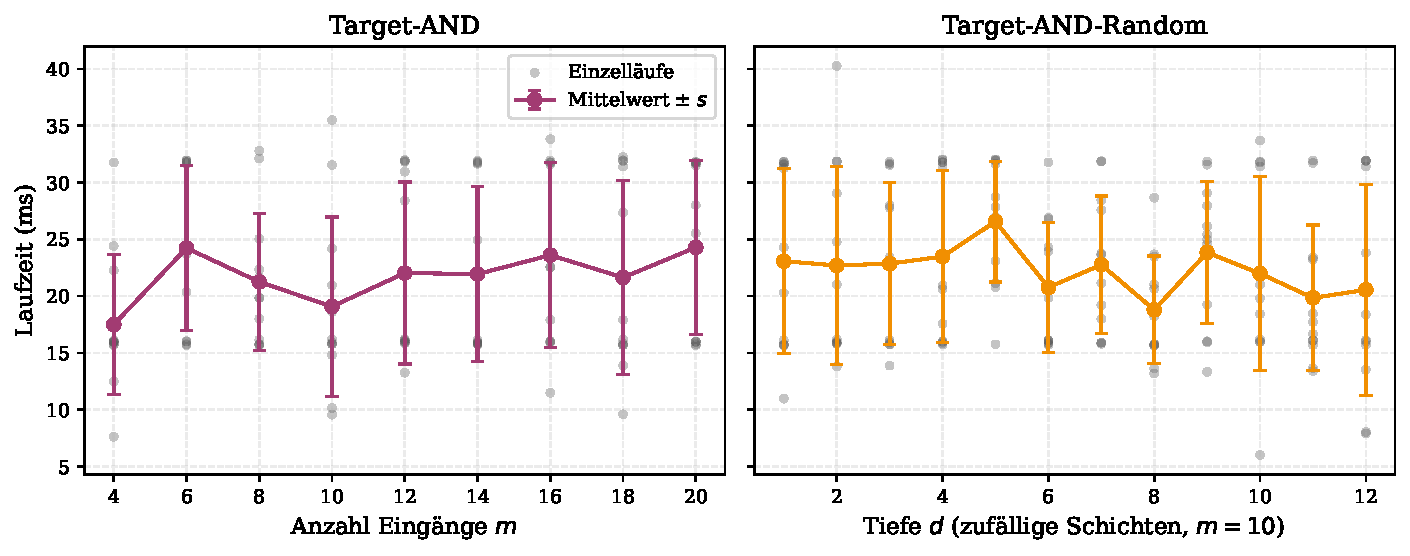
\includegraphics[width=\textwidth]{fig_parameters.pdf}
\caption{Laufzeit in Abhängigkeit von der Eingangszahl $m$ (links, Target-AND) und der Tiefe $d$ (rechts, Target-AND-Random mit $m=10$); beide Teilbilder teilen sich die Ordinate. Graue Punkte: Einzelläufe (je 12 pro Abszissenwert); farbige Punkte mit Linienzug: Mittelwert; senkrechte Balken: Mittelwert $\pm$ eine Standardabweichung.}
\label{fig:param}
\end{figure}

\paragraph{Aufbau der Abbildung.} Abbildung~\ref{fig:param} besteht aus zwei nebeneinanderliegenden Teilbildern mit gemeinsamer Ordinate (Laufzeit in ms, etwa von $5$ bis $42$\,ms). Im linken Teilbild ist die Eingangszahl $m = 4, 6, \ldots, 20$ der Target-AND-Circuits auf der Abszisse aufgetragen (neun Positionen, entsprechend $7$ bis $39$ Gates), im rechten die Tiefe $d = 1, \ldots, 12$ der Target-AND-Random-Circuits bei festem $m = 10$ (zwölf Positionen, entsprechend $27$ bis $54$ Gates). An jeder Position sind alle $12$ Einzelläufe als halbtransparente graue Punkte eingezeichnet; wo mehrere Läufe nahezu denselben Wert haben, überlagern sich die Punkte und erscheinen dunkler. Darüber liegt jeweils ein farbiger Punkt für den Mittelwert (links violett, rechts orange), der durch einen Linienzug mit den Nachbarpositionen verbunden ist, sowie ein senkrechter Balken mit Querstrichen, der von $\bar{t} - s$ bis $\bar{t} + s$ reicht. Die Legende steht nur im linken Teilbild.

\paragraph{Linkes Teilbild: Target-AND.} Der Linienzug verläuft nicht monoton. Er beginnt mit dem kleinsten Mittelwert bei $m = 4$ ($17{,}49$\,ms), springt bei $m = 6$ auf $24{,}23$\,ms, fällt über $21{,}25$\,ms ($m = 8$) auf ein Nebenminimum von $19{,}09$\,ms bei $m = 10$, bewegt sich danach zwischen $21{,}6$ und $23{,}6$\,ms und erreicht bei $m = 20$ mit $24{,}29$\,ms seinen höchsten Wert. Über den gesamten Bereich, in dem die Instanz von $7$ auf $39$ Gates wächst, ändert sich der Mittelwert damit um höchstens $6{,}8$\,ms, also um weniger als eine Standardabweichung. Die Balken sind mit $s = 6{,}02$ bis $8{,}56$\,ms so lang, dass sich alle neun überlappen; der Balken bei $m = 4$ reicht beispielsweise von $11{,}35$ bis $23{,}63$\,ms, der bei $m = 20$ von $16{,}64$ bis $31{,}94$\,ms. Die grauen Punkte zeigen, woher die Streuung stammt: An fast jeder Eingangszahl liegt ein Teil der Läufe in einem schmalen Band bei $15{,}6$ bis $16$\,ms, ein anderer Teil in einem Band bei etwa $31{,}7$ bis $32$\,ms. Der Mittelwert fällt deshalb meist in die Lücke zwischen den beiden Bändern, in der nur wenige Einzelwerte liegen. Aus demselben Grund sind die Balken nicht als Konfidenzintervall zu lesen: Bei einer zweigipfligen Verteilung beschreibt $\bar{t} \pm s$ keinen Bereich, in dem die Läufe typischerweise liegen. Die Extremwerte sind $7{,}62$\,ms ($m = 4$) und $35{,}50$\,ms ($m = 10$). Ein mit $m$ ansteigender Verlauf, wie ihn eine wachsende Instanz erwarten ließe, ist nicht erkennbar. Da bei Target-AND die Gate-Anzahl $2m-1$ beträgt, ist die Rangkorrelation mit $m$ identisch zu der mit der Gate-Anzahl ($\rho = 0{,}106$, $p = 0{,}275$).

\paragraph{Rechtes Teilbild: Target-AND-Random.} Auch hier ist der Linienzug unsystematisch. Die Mittelwerte liegen für $d = 1$ bis $4$ nahezu auf einem Plateau ($22{,}70$ bis $23{,}48$\,ms), erreichen bei $d = 5$ ihr Maximum von $26{,}57$\,ms, fallen bei $d = 6$ auf $20{,}77$\,ms, steigen bei $d = 7$ und $d = 9$ wieder auf rund $23$ bis $24$\,ms und haben bei $d = 8$ ihr Minimum von $18{,}79$\,ms. Für $d = 10$ bis $12$ liegen sie zwischen $19{,}85$ und $21{,}99$\,ms, also im Mittel unter dem Plateau der kleinen Tiefen; bei $d = 12$ ($20{,}56$\,ms) ist der Mittelwert um $2{,}52$\,ms kleiner als bei $d = 1$ ($23{,}08$\,ms), obwohl der Circuit dann doppelt so viele Gates hat. Die Extrema lassen sich an den Einzelpunkten nachvollziehen: Bei $d = 5$ liegt mehr als die Hälfte der Läufe oberhalb von $27{,}4$\,ms (Median $27{,}43$\,ms), bei $d = 8$ erreicht dagegen kein Lauf das obere Band (Maximum $28{,}66$\,ms), was den niedrigsten Mittelwert erklärt. Die tiefsten Einzelwerte der gesamten Studie stehen bei $d = 10$ ($6{,}02$\,ms) und $d = 12$ ($7{,}91$\,ms), der höchste ($40{,}27$\,ms) bei $d = 2$. Die Balken ($s = 4{,}74$ bis $9{,}30$\,ms) überlappen ebenfalls durchgehend. Die lineare Regression ergibt $-0{,}28$\,ms pro Schicht; über alle elf Tiefenschritte wären das $-3{,}0$\,ms, etwa $0{,}4$ Standardabweichungen aller Läufe. Da die Zwischenschichten mit festem Seed erzeugt werden, ist jeder Circuit deterministisch. Die Streuung innerhalb einer Tiefe ist daher reines Messrauschen und keine Variation zwischen verschiedenen Zufallscircuits.

\paragraph{Gesamtbild.} In beiden Teilbildern bewegen sich die Mittelwerte im selben Band von etwa $17$ bis $27$\,ms, und in beiden bilden die grauen Punkte dieselben zwei horizontalen Bänder bei $15{,}6$ und $31{,}7$\,ms. Die Teilbilder unterscheiden sich damit weder in der Höhe noch in der Form der Streuung, obwohl links die Eingangszahl und rechts die Schichtenzahl variiert wird. Aus Abbildung~\ref{fig:param} lässt sich daher kein Einfluss von $m$ oder $d$ auf die gemessene Laufzeit ablesen.

\subsection{ISCAS'85-Benchmarks (F3)}

Alle zwölf ISCAS'85-Circuits wurden in der Standard-, der Full- und der Performance-Suite je einmal ausgeführt (je Circuit $n=3$, Tabelle~\ref{tab:iscas}). Die Instanzen reichen von $4$ bis $3\,512$ Gates. Die mittleren Laufzeiten liegen zwischen $15{,}79$\,ms (c3540) und $31{,}85$\,ms (c1355). Der größte Circuit c7552 (3\,512 Gates, 10\,690 Klauseln) wird mit im Mittel $21{,}26$\,ms gelöst und ist damit nicht langsamer als der Mittelwert über alle ISCAS-Läufe ($20{,}23$\,ms). Die Korrelation zwischen Gate-Anzahl und Laufzeit ist je Suite schwach und nicht signifikant (Standard: $r = 0{,}37$, $p = 0{,}24$; Full: $r = -0{,}18$, $p = 0{,}58$; Performance: $r = -0{,}20$, $p = 0{,}53$); über alle 36 ISCAS-Läufe gilt $\rho = 0{,}104$ ($p = 0{,}547$).

\begin{table}[ht]
\centering\small
\input{\resultsdir/paper/tab_iscas.tex}
\caption{ISCAS'85: Struktur und Laufzeit (ms) je Circuit, aufsteigend nach Größe. Je Circuit $n=3$ Läufe (Standard, Full, Performance).}
\label{tab:iscas}
\end{table}

\begin{figure}[ht]
\centering
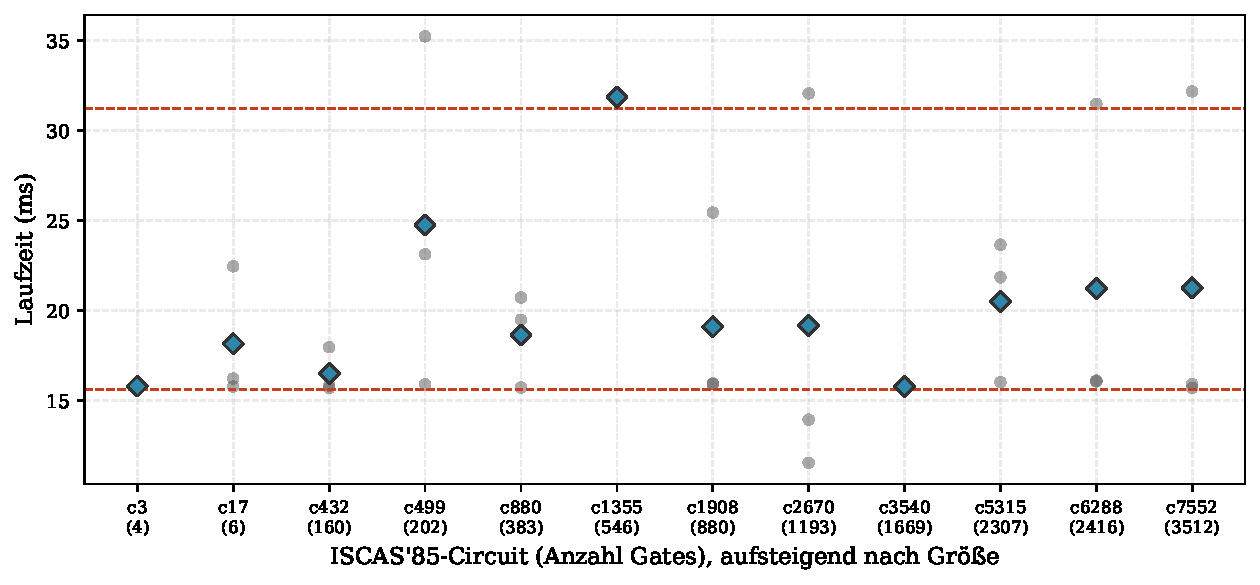
\includegraphics[width=0.95\textwidth]{fig_iscas.pdf}
\caption{ISCAS'85: Einzelläufe (graue Punkte, je Circuit drei) und Mittelwert (blaue Raute) je Circuit. Die Circuits stehen in gleichen Abständen, aufsteigend nach Gate-Anzahl (in Klammern). Gestrichelt: $15{,}625$\,ms und $31{,}25$\,ms.}
\label{fig:iscas}
\end{figure}

\paragraph{Aufbau der Abbildung.} Abbildung~\ref{fig:iscas} zeigt für jeden der zwölf ISCAS'85-Circuits die drei Einzelläufe (Standard, Full, Performance). Die Abszisse ist kategorial: Die Circuits stehen in gleichen Abständen, aufsteigend nach Gate-Anzahl von c3 ($4$ Gates) bis c7552 ($3\,512$ Gates); der Abstand zweier Positionen ist daher \emph{nicht} proportional zum Größenunterschied. Unter jedem Namen steht in Klammern die Gate-Anzahl. Die Ordinate gibt die Laufzeit in ms an. Die drei Läufe eines Circuits sind graue, halbtransparente Punkte direkt übereinander; fallen Werte zusammen, verschmelzen sie zu einem einzigen, dunkleren Punkt. Die blaue Raute markiert den Mittelwert, die beiden gestrichelten horizontalen Linien liegen bei $15{,}625$ und $31{,}25$\,ms.

\paragraph{Lesart.} Bei c3 und c3540 liegen alle drei Punkte praktisch übereinander auf der unteren Linie ($15{,}75$ bis $15{,}88$\,ms bzw.\ $15{,}67$ bis $16{,}00$\,ms); die Raute sitzt dort bei $15{,}80$ bzw.\ $15{,}79$\,ms. Das ist bemerkenswert, weil zwischen diesen beiden Circuits ein Faktor $417$ in der Gate-Anzahl liegt ($4$ gegenüber $1\,669$). Bei zehn der zwölf Circuits liegt der kleinste der drei Werte zwischen $15{,}67$ und $16{,}06$\,ms, also auf oder knapp über der unteren Linie, unabhängig davon, ob der Circuit $4$ oder $3\,512$ Gates hat. Die beiden Ausnahmen sind c1355 (kleinster Wert $31{,}69$\,ms) und c2670 ($11{,}54$\,ms, unterhalb der unteren Linie). Eine zweite Gruppe von Punkten liegt auf oder nahe der oberen Linie: je ein Lauf bei c2670 ($32{,}06$\,ms), c6288 ($31{,}49$\,ms) und c7552 ($32{,}18$\,ms) sowie alle drei Läufe von c1355. Insgesamt liegen $19$ der $36$ Werte innerhalb von $\pm 1$\,ms um die untere und $6$ innerhalb von $\pm 1$\,ms um die obere Linie.

Die größte Spannweite innerhalb eines Circuits haben c2670 ($11{,}54$ bis $32{,}06$\,ms, $20{,}5$\,ms) und c499 ($15{,}90$ bis $35{,}24$\,ms, $19{,}3$\,ms). Der Wert $35{,}24$\,ms bei c499 ist der einzige ISCAS-Lauf deutlich oberhalb der oberen Linie. Dadurch liegt die Raute von c499 ($24{,}75$\,ms) höher als die der größeren Circuits c880 ($18{,}64$\,ms) und c1908 ($19{,}10$\,ms). Die Rauten der drei größten Circuits c5315, c6288 und c7552 liegen bei $20{,}51$, $21{,}22$ und $21{,}26$\,ms und damit auf demselben Niveau wie die der mittleren Circuits c880 bis c2670 ($18{,}64$ bis $19{,}18$\,ms). Von links nach rechts ist in der Folge der Rauten keine steigende Tendenz erkennbar.

\paragraph{Zusammenfassung des Bildes.} Weder die Lage der Einzelpunkte noch die der Rauten ordnet sich nach der Gate-Anzahl. Die Punkte der größten Circuits rechts im Bild liegen im selben Wertebereich wie die der kleinsten links; ihre Streuung ist dabei teils größer als die der kleinen Circuits, jedoch ohne klare Ordnung. Das Bild zeigt damit dieselben zwei Bänder bei $15{,}625$ und $31{,}25$\,ms wie Abbildung~\ref{fig:hist}.

Auffällig ist c1355: In allen drei Läufen liegt die Laufzeit bei $31{,}69$ bis $32{,}00$\,ms (Standardabweichung $0{,}16$\,ms), während die kleinere Instanz c880 (383 Gates) und die größere Instanz c1908 (880 Gates) im Mittel nur $18{,}64$\,ms bzw.\ $19{,}10$\,ms benötigen. Es ist der einzige Circuit mit einer in allen Wiederholungen übereinstimmend erhöhten Laufzeit. Mit nur drei Wiederholungen und der in Abschnitt~\ref{sec:zeit} beschriebenen Messauflösung lässt sich nicht entscheiden, ob dies auf eine strukturelle Eigenschaft der Instanz oder auf Zufall zurückgeht. Auch die Funktion von c1355 als NAND-Variante von c499 (mit $24{,}75$\,ms im Mittel) liefert dafür keine eindeutige Erklärung.

\subsection{Zusammenhang zwischen Instanzgröße und Laufzeit}

Tabelle~\ref{tab:correlation} fasst die Zusammenhangsmaße zusammen. Über alle 288 Läufe beträgt die Rangkorrelation zwischen Gate-Anzahl und Laufzeit $\rho = 0{,}024$ ($p = 0{,}686$); die lineare Regression ergibt eine Steigung von $-0{,}6$\,$\mu$s pro Gate bei $R^2 = 0{,}002$. In keiner Teilmenge ist ein Zusammenhang signifikant ($p > 0{,}1$ in allen Fällen), und die Bestimmtheitsmaße liegen unter $2{,}5\,\%$. Abbildung~\ref{fig:gates} zeigt dies grafisch: Über mehr als zwei Größenordnungen der Gate-Anzahl verteilen sich die Laufzeiten im selben Band zwischen etwa $6$ und $40$\,ms.

\begin{table}[ht]
\centering\footnotesize
\setlength{\tabcolsep}{3.5pt}
\input{\resultsdir/paper/tab_correlation.tex}
\caption{Zusammenhang zwischen Instanzgröße (Gates bzw.\ Tiefe) und Laufzeit. $\rho$: Spearman, $r$: Pearson, jeweils mit $p$-Wert; Steigung und $R^2$ aus der linearen Regression der Laufzeit auf die Gate-Anzahl.}
\label{tab:correlation}
\end{table}

\begin{figure}[ht]
\centering
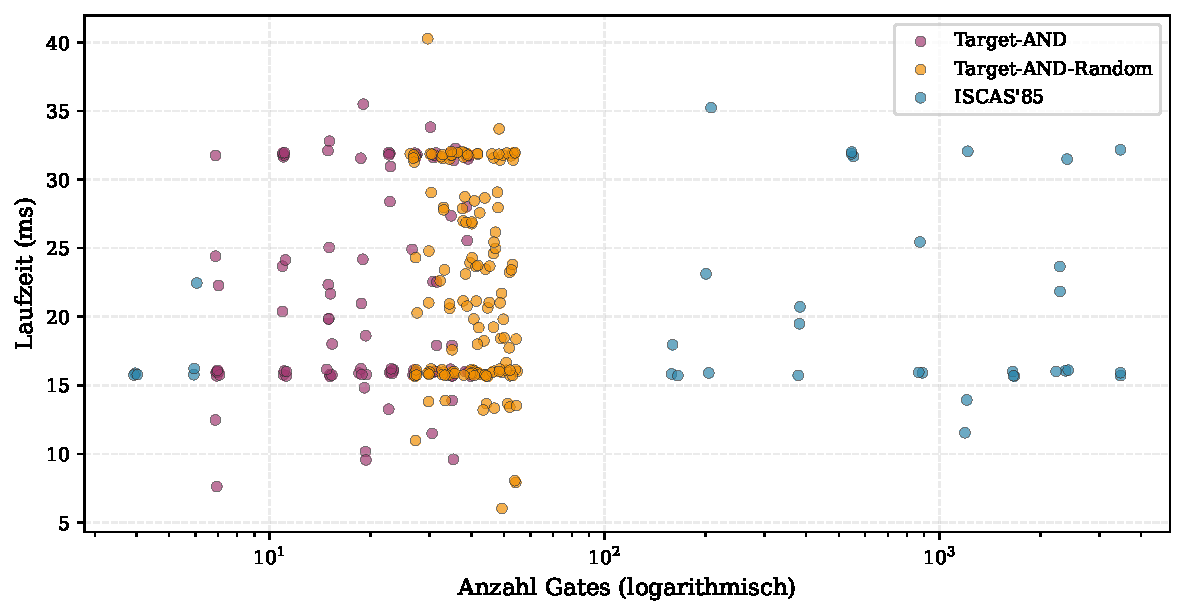
\includegraphics[width=0.95\textwidth]{fig_gates_vs_runtime.pdf}
\caption{Laufzeit gegen Gate-Anzahl für alle 288 Läufe (logarithmische Abszisse, leichte horizontale Streuung der Punkte zur besseren Lesbarkeit). Violett: Target-AND, orange: Target-AND-Random, blau: ISCAS'85.}
\label{fig:gates}
\end{figure}

\paragraph{Aufbau der Abbildung.} Abbildung~\ref{fig:gates} ist ein Streudiagramm, in dem jeder der $288$ Läufe ein Punkt ist. Die Abszisse zeigt die Gate-Anzahl auf logarithmischer Skala (von $4$ bis $3\,512$, knapp drei Größenordnungen), die Ordinate die Laufzeit in ms (linear, etwa von $5$ bis $42$\,ms). Die Farbe kodiert den Circuit-Typ: Target-AND violett, Target-AND-Random orange, ISCAS'85 blau. Die Punkte sind halbtransparent. Weil viele Läufe dieselbe Gate-Anzahl haben (jeder Circuit wird bis zu fünfmal ausgeführt), wurde jeder Punkt horizontal um etwa $1\,\%$ der Abszisse zufällig verschoben; ein Punkt steht daher nur ungefähr über seiner Gate-Anzahl. Eine Ausgleichsgerade ist nicht eingezeichnet.

\paragraph{Die drei Punktwolken.} Die Typen belegen verschiedene Abschnitte der Abszisse. Die Target-AND-Läufe (violett) liegen zwischen $7$ und $39$ Gates, die Target-AND-Random-Läufe (orange) zwischen $27$ und $54$ Gates und bilden eine dichte, schmale Säule; beide überlappen im Bereich von $27$ bis $39$ Gates. Oberhalb von $100$ Gates liegen ausschließlich ISCAS-Läufe (blau): zehn Circuits mit zusammen $30$ Läufen bis $3\,512$ Gates. Die übrigen sechs ISCAS-Läufe (c3 und c17) liegen bei $4$ bis $6$ Gates links von allen synthetischen Läufen. Die Ordinatenwerte aller drei Wolken liegen im selben Bereich: bei Target-AND von $7{,}62$ bis $35{,}50$\,ms, bei ISCAS\'85 von $11{,}54$ bis $35{,}24$\,ms und bei Target-AND-Random von $6{,}02$ bis $40{,}27$\,ms. Der höchste Punkt des Diagramms ist der Einzelwert $40{,}27$\,ms bei $30$ Gates (orange); die tiefsten Punkte sind $6{,}02$ und $7{,}91$\,ms bei $49$ bzw.\ $54$ Gates (ebenfalls orange).

\paragraph{Horizontale Bänder statt Anstieg.} Auffällig sind zwei horizontale Bänder, auf denen sich die Punkte häufen: eines bei etwa $15{,}6$ bis $16$\,ms und eines bei etwa $31{,}5$ bis $32$\,ms. Beide ziehen sich über die gesamte Abszisse. Im unteren Band liegen die ISCAS-Punkte von c3 ($4$ Gates) bis c7552 ($3\,512$ Gates), im oberen finden sich sieben ISCAS-Läufe bei $30$\,ms und mehr (unter anderem c1355 mit $546$ Gates und c7552 mit $3\,512$ Gates). Zwischen den Bändern liegt ein dünner besiedelter Bereich, der überwiegend von den orangen Punkten gefüllt wird. Würde die Laufzeit mit der Instanzgröße wachsen, wäre eine von links unten nach rechts oben ansteigende Punktwolke zu erwarten; das Bild zeigt stattdessen, dass die Punkte rechts (bis $3\,512$ Gates) nicht höher liegen als links. Das deckt sich mit den Maßzahlen ($\rho = 0{,}024$ über alle Läufe, Tabelle~\ref{tab:correlation}). Weil zwischen den größten und kleinsten Instanzen derselbe Wertebereich liegt, bildet die Ordinate hier offenbar nicht die Lösungszeit ab, sondern die in Abschnitt~\ref{sec:zeit} beschriebene Messgrundlast.

\subsection{Vergleich der Circuit-Typen und der Suites (F4)}

Die Circuit-Typen unterscheiden sich in ihrer Laufzeit nicht signifikant (Kruskal--Wallis: $H = 2{,}63$, $p = 0{,}268$); ebenso wenig die Gruppe der ISCAS-Läufe von den synthetischen Läufen (Mann--Whitney: $p = 0{,}140$). Auch zwischen den vier Suites besteht kein signifikanter Unterschied ($H = 2{,}39$, $p = 0{,}495$, Tabelle~\ref{tab:tests}). Die Mittelwerte über die gesamte Suite betragen $24{,}52$\,ms (Quick), $22{,}46$\,ms (Standard), $21{,}68$\,ms (Full) und $21{,}27$\,ms (Performance); die Tendenz zu kleineren Mittelwerten bei größeren Suites ist mit den kleinen Stichproben der Quick-Suite ($n=21$) vereinbar.

Der direkte Vergleich der beiden gleich aufgebauten Suites Full und Performance (Tabelle~\ref{tab:full_vs_perf}) zeigt Abweichungen der Mittelwerte von $+2{,}8$\,\%, $-5{,}6$\,\% und $+0{,}7$\,\% für die drei Circuit-Typen; keiner dieser Unterschiede ist signifikant ($p = 0{,}513$, $0{,}483$ und $0{,}751$).

\begin{table}[ht]
\centering\small
\input{\resultsdir/paper/tab_full_vs_perf.tex}
\caption{Vergleich der Suites Full und Performance (identische Zusammensetzung). Mittelwerte $\bar{t}$ und Standardabweichungen $s$ in ms.}
\label{tab:full_vs_perf}
\end{table}

\begin{table}[ht]
\centering\small
\input{\resultsdir/paper/tab_tests.tex}
\caption{Ergebnisse der Rangtests. Alle $p$-Werte liegen deutlich über $\alpha = 0{,}05$.}
\label{tab:tests}
\end{table}

\begin{figure}[ht]
\centering
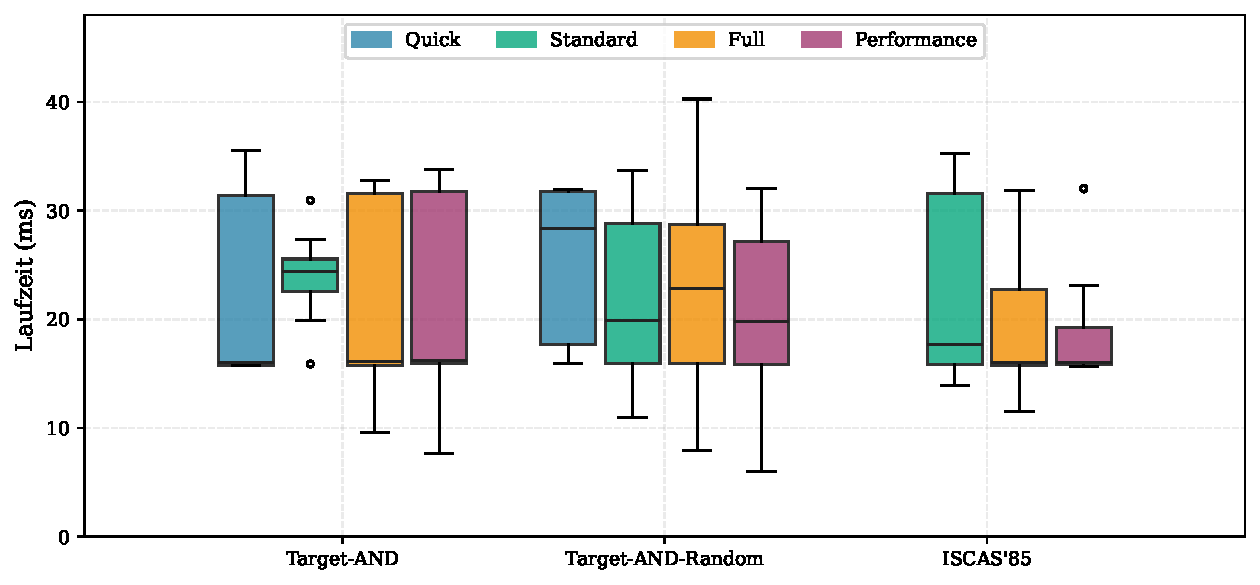
\includegraphics[width=0.95\textwidth]{fig_suites.pdf}
\caption{Boxplots der Laufzeit je Circuit-Typ (Gruppen) und Suite (innerhalb jeder Gruppe von links nach rechts: Quick blau, Standard grün, Full orange, Performance violett). Box: erstes bis drittes Quartil; Querstrich: Median; Whisker: äußerste Werte innerhalb des 1,5-fachen Interquartilsabstands; Kreise: Werte außerhalb. Für ISCAS'85 fehlt Quick (keine ISCAS-Läufe).}
\label{fig:suites}
\end{figure}

\paragraph{Aufbau der Abbildung.} Abbildung~\ref{fig:suites} fasst die Laufzeitverteilung je Suite und Circuit-Typ in Boxplots zusammen (die zugehörigen Zahlen stehen in Tabelle~\ref{tab:suite_type}). Die Abszisse ist in drei Gruppen geteilt: Target-AND, Target-AND-Random und ISCAS'85. Innerhalb jeder Gruppe stehen von links nach rechts bis zu vier Boxen für die Suites Quick (blau), Standard (grün), Full (orange) und Performance (violett). Eine Box reicht vom ersten bis zum dritten Quartil und enthält damit die mittleren $50\,\%$ der Läufe; der schwarze Querstrich ist der Median. Die Whisker reichen bis zum äußersten Wert innerhalb des $1{,}5$-fachen Interquartilsabstands, Werte außerhalb sind als kleine Kreise dargestellt. Die Ordinate zeigt die Laufzeit von $0$ bis $48$\,ms. In der Gruppe ISCAS'85 fehlt die Quick-Box, weil Quick keine ISCAS-Circuits enthält (Tabelle~\ref{tab:suites}); dort stehen nur drei Boxen, und die linke Position bleibt leer.

\paragraph{Target-AND.} Die Boxen von Quick, Full und Performance sehen sich sehr ähnlich: Die Box reicht von rund $15{,}8$\,ms ($Q_1 = 15{,}77$ bis $15{,}90$\,ms) bis rund $31{,}5$\,ms ($Q_3 = 31{,}40$ bis $31{,}74$\,ms), und der Median liegt bei $16{,}00$, $16{,}11$ bzw.\ $16{,}20$\,ms unmittelbar am unteren Boxrand. Die Boxen sind also stark asymmetrisch: Mehr als die Hälfte der Läufe liegt im unteren Band, die obere Hälfte der Box ist dagegen sehr lang. Die Whisker reichen bei Full von $9{,}60$ bis $32{,}80$\,ms, bei Performance von $7{,}62$ bis $33{,}83$\,ms und bei Quick bis $35{,}50$\,ms. Abweichend ist nur Standard: Die Box ist schmal ($22{,}56$ bis $25{,}55$\,ms, Median $24{,}41$\,ms), und zwei Werte ($15{,}89$ und $30{,}96$\,ms) werden als Kreise abgesetzt. Dieser Unterschied beruht auf nur neun Läufen; zugleich ist es die Zelle mit der kleinsten Standardabweichung aller elf Kombinationen ($s = 4{,}30$\,ms). Der Kruskal--Wallis-Test über alle Suites findet keinen signifikanten Unterschied ($p = 0{,}495$).

\paragraph{Target-AND-Random.} Bei den zufälligen Circuits beginnen alle vier Boxen nahe dem unteren Band ($Q_1 = 15{,}84$ bis $15{,}96$\,ms; nur bei Quick $17{,}68$\,ms) und enden zwischen $27{,}12$\,ms (Performance) und $31{,}77$\,ms (Quick). Die Mediane streuen stärker als in den anderen Gruppen: Quick $28{,}32$\,ms, Standard $19{,}92$\,ms, Full $22{,}87$\,ms und Performance $19{,}83$\,ms. Der hohe Quick-Median ist der größte aller elf Mediane. Er liegt in der Lücke zwischen den beiden Bändern, wo die Dichte der Läufe gering ist; bei einer zweigipfligen Verteilung genügt dann die Verschiebung weniger Läufe zwischen den Bändern, um den Median stark zu verändern. Die Whisker von Full ($7{,}91$ bis $40{,}27$\,ms) und Performance ($6{,}02$ bis $32{,}05$\,ms) enthalten die Extremwerte der gesamten Studie.

\paragraph{ISCAS'85.} Bei Full und Performance sind die Boxen verhältnismäßig schmal ($15{,}74$ bis $22{,}76$\,ms bzw.\ $15{,}88$ bis $19{,}25$\,ms), und die Mediane liegen mit $16{,}03$ und $16{,}06$\,ms am unteren Band; bei Performance ist ein Lauf mit $32{,}06$\,ms als Kreis abgesetzt. Die Standard-Box ist deutlich breiter ($15{,}81$ bis $31{,}54$\,ms, Median $17{,}70$\,ms, Whisker $13{,}93$ bis $35{,}24$\,ms). In allen drei Suites liegen die ISCAS-Boxen nicht oberhalb der Boxen der kleinen synthetischen Circuits, obwohl die ISCAS-Instanzen bis zu etwa $90$-mal mehr Gates haben als die Target-AND-Circuits.

\paragraph{Gesamtbild.} Alle elf Boxen liegen zwischen $15{,}74$ und $31{,}77$\,ms; ihre Mediane liegen zwischen $16{,}00$ und $28{,}32$\,ms. Weder ordnen sich die vier Suitefarben innerhalb einer Gruppe systematisch (etwa aufsteigend), noch unterscheiden sich die drei Gruppen in Lage oder Form. Das entspricht den Rangtests in Tabelle~\ref{tab:tests} und dem Vergleich von Full und Performance in Tabelle~\ref{tab:full_vs_perf}. Die Unterschiede zwischen den Boxen sind kleiner als die Streuung innerhalb jeder einzelnen Box.

\subsection{Zeitliche Auflösung der Messung}
\label{sec:zeit}

Tabelle~\ref{tab:quant} zeigt die Verteilung der Laufzeiten in Klassen. $105$ der $288$ Werte ($36{,}5\,\%$) liegen zwischen $15{,}0$ und $16{,}5$\,ms und weitere $68$ ($23{,}6\,\%$) zwischen $31{,}0$ und $33{,}0$\,ms. Insgesamt liegen $173$ Werte ($60{,}1\,\%$) innerhalb von $\pm 1$\,ms um $15{,}625$\,ms oder $31{,}25$\,ms. Bei einer gleichmäßigen Verteilung über den beobachteten Bereich von $6$ bis $40$\,ms wären für diese beiden Fenster nur etwa $12\,\%$ der Werte zu erwarten.

Der Wert $15{,}625\,\mathrm{ms} = 1/64\,\mathrm{s}$ entspricht der typischen Aktualisierungsrate der Systemuhr unter Windows. Die auffällige Häufung bei diesem Wert und seinem Doppelten ist daher konsistent mit einer groben Zeitauflösung von \texttt{time.time()}. Die Werte dazwischen (etwa 40\,\%) zeigen, dass die Auflösung nicht in allen Läufen gleich grob war. Wir behandeln diese Erklärung als gut gestützte Hypothese, nicht als bewiesen; der Datensatz enthält keine Information über Betriebssystem oder Uhr.

\begin{table}[ht]
\centering\small
\input{\resultsdir/paper/tab_quantization.tex}
\caption{Häufigkeit der Laufzeiten in Klassen über alle 288 Läufe.}
\label{tab:quant}
\end{table}

\subsection{Solver-Ausgabe und Erfüllbarkeit}

In keinem der 288 Läufe wurde ein Erfüllbarkeitsergebnis erfasst: Das Feld \texttt{satisfiable} ist durchgehend \texttt{False}, das Feld \texttt{solver\_output} stets leer, und es wurde kein Fehler protokolliert. Der Solver-Prozess wurde also gestartet und beendete sich ohne Ausgabe auf Standardausgabe und Fehlerausgabe, ohne dass der Runner den Rückgabecode ausgewertet hätte. Dieser Befund steht im Widerspruch zu der in Abschnitt~\ref{sec:cnf} gezeigten Eigenschaft, dass die erzeugten Formeln erfüllbar sind. Er wird in Abschnitt~\ref{sec:diskussion} bewertet.

%=====================================================================
\section{Diskussion}
\label{sec:diskussion}

\subsection{Was die Daten stützen}

\begin{itemize}
	\item \textbf{Keine Größenabhängigkeit im gemessenen Bereich.} Weder Gate-Anzahl, Klauselzahl, Eingangszahl noch Tiefe erklären die Laufzeit; alle Korrelationen sind schwach ($|\rho| \le 0{,}11$) und nicht signifikant. Dies gilt über einen Größenbereich von $4$ bis $3\,512$ Gates.
	\item \textbf{Kein Typ-Effekt.} ISCAS'85 mit durchschnittlich $1\,106{,}5$ Gates wird nicht langsamer verarbeitet als Target-AND mit durchschnittlich $23{,}0$ Gates.
	\item \textbf{Konsistenz der Messungen.} Die Suites unterscheiden sich nicht signifikant, und Full und Performance liefern im Mittel dieselben Ergebnisse.
	\item \textbf{Stabilität.} Alle Läufe endeten ohne Timeout (30\,s) und ohne Fehlermeldung; die maximale Laufzeit beträgt $40{,}27$\,ms.
\end{itemize}

\subsection{Was die Daten nicht stützen}

Eine Beobachtung der Form \glqq die Laufzeit ist nicht von der Größe abhängig\grqq{} ist nur dann eine Aussage über den \emph{Algorithmus}, wenn die gemessene Zeit tatsächlich die Rechenzeit des Algorithmus widerspiegelt. Dies ist hier aus vier Gründen nicht gesichert:

\begin{enumerate}
	\item \textbf{Der Messwert wird vom Prozessstart dominiert.} Der häufigste Messwert liegt bei etwa $16$\,ms, und die Werte ändern sich nicht, wenn die Instanz um den Faktor $878$ wächst: Der kleinste ISCAS-Circuit c3 (4 Gates) und der größte, c7552 (3\,512 Gates), erreichen beide ein Minimum von etwa $15{,}7$ bis $15{,}8$\,ms. Plausibel ist, dass die gemessene Zeit im Wesentlichen aus Prozessstart, Datei-I/O und Laufzeitumgebung besteht und die eigentliche Lösungszeit darunter liegt. Die Messung liefert dann eine obere Schranke der Solver-Zeit, aber keine Skalierungsinformation.
	\item \textbf{Die Zeitauflösung ist grob} (Abschnitt~\ref{sec:zeit}). Der mehrgipfelige Verlauf der Verteilung, die in früheren Auswertungen als bimodale Verteilung langsamer und schneller Instanzen gedeutet wurde, ist mit einem Messartefakt gut vereinbar.
	\item \textbf{Es wurde keine Solver-Ausgabe erfasst.} Weil für keinen Lauf ein SAT/UNSAT-Ergebnis vorliegt, ist nicht belegt, dass der Solver die Instanzen tatsächlich gelöst hat. Da die erzeugten Formeln erfüllbar sind (keine Unit-Klausel auf dem Ausgang, Abschnitt~\ref{sec:cnf}), müsste ein korrekt arbeitender Solver \texttt{SAT} melden; das durchgehend leere Ergebnis spricht dafür, dass entweder der Solver keine oder eine nicht erkannte Ausgabe erzeugt oder dass er die Eingabe nicht verarbeitet. Der Runner prüft den Rückgabecode des Prozesses nicht.
	\item \textbf{Die Kodierung ist für NAND, NOR und XOR fehlerhaft} (Abschnitt~\ref{sec:cnf}). Die ISCAS'85-Läufe messen daher den Solver auf Formeln, die nicht die ISCAS-Circuits darstellen. Strukturell bleiben sie in Größe und Klauselzahl vergleichbar, ihr logischer Inhalt ist jedoch ein anderer.
\end{enumerate}

Aus diesen Gründen können die Experimente weder die theoretische Laufzeit $\Theta(n^3)$ des Subgraph Algorithmus bestätigen noch widerlegen. Insbesondere ist die Aussage eines sublinearen oder konstanten Skalierungsverhaltens \emph{nicht} aus den Daten ableitbar: Konstanz im Rauschen einer Prozessstart-dominierten Messung ist keine Konstanz des Algorithmus. Das gilt ebenso für Aussagen über einen tiefenabhängigen Anstieg, eine ISCAS-spezifische Beschleunigung oder nichtmonotones Laufzeitverhalten (etwa c1355): All dies liegt im Rahmen des Messrauschens bzw.\ lässt sich mit drei Wiederholungen je Circuit nicht absichern.

\subsection{Gültigkeitsbedrohungen}

\begin{itemize}
	\item \textbf{Interne Validität.} \texttt{time.time()} ist keine monotone, hochauflösende Uhr; \texttt{time.perf\_counter()} wäre geeigneter. Pro Instanz gibt es 1 bis 12 Wiederholungen ohne Aufwärmphase und ohne Berücksichtigung von Cache- und Betriebssystemeffekten.
	\item \textbf{Konstruktvalidität.} Gemessen wird die Wallclock-Zeit eines Prozesses, nicht die Rechenzeit des Algorithmus. Das Erfüllbarkeitsergebnis ist nicht erfasst (s.\,o.). Die Kodierung von NAND, NOR und XOR ist fehlerhaft. Der Speicherverbrauch wird nicht gemessen.
	\item \textbf{Externe Validität.} Die erzeugten Instanzen sind erfüllbar und strukturell einfach (Target-AND ist ein einzelner AND-Baum); die ISCAS-Formeln enthalten ebenfalls keine Ausgangsbedingung. Es gibt keine unerfüllbaren Instanzen und keinen Vergleich mit etablierten SAT-Solvern.
	\item \textbf{Umgebung.} Der Datensatz enthält keine Angaben zu Betriebssystem, Hardware, Python-Version oder Solver-Version.
\end{itemize}

\subsection{Verbesserungen des Messaufbaus}

Wir schlagen vor, die folgenden Änderungen am Framework vorzunehmen und die Experimente zu wiederholen:
\begin{enumerate}
	\item Korrektur der Tseitin-Kodierung für NAND, NOR und XOR und Test der Kodierung gegen die Wahrheitstabelle jedes Gate-Typs.
	\item Auswertung von Rückgabecode und Ausgabe des Solvers; Erfassen von SAT/UNSAT und gegebenenfalls der Belegung; Prüfen der Belegung gegen den Circuit.
	\item Verwendung von \texttt{time.perf\_counter()} und, falls vom Solver unterstützt, einer solverinternen Zeitmessung; zusätzlich Messung der Prozessstart-Grundlast mit einer trivialen Instanz.
	\item Mehr Wiederholungen je Instanz (z.\,B.\ $\ge 30$) mit Aufwärmläufen sowie Angabe von Median und Konfidenzintervall.
	\item Instanzen mit Unit-Klausel auf dem Ausgang, unerfüllbare Instanzen und deutlich größere Circuits ($10^4$ bis $10^5$ Gates), damit ein Skalierungseffekt über das Messrauschen hinauswächst.
	\item Erfassen von Betriebssystem, Hardware, Python- und Solver-Version sowie Messung des Speicherverbrauchs.
	\item Vergleich mit etablierten Solvern (z.\,B.\ MiniSat, CaDiCaL) auf denselben CNF-Dateien.
\end{enumerate}

%=====================================================================
\section{Neue Version der Experimente (Version 2.0.0)}
\label{sec:v2}

\noindent\fbox{\parbox{0.96\textwidth}{\small\textbf{Hinweis.} Dieser Abschnitt berichtet über die \emph{neue Version der Experimente}. Sie wurde mit der Version~2.0.0 der Python-Module des Frameworks (\texttt{subgraph-sat-solver-experiments}, \texttt{version = "2.0.0"} in \texttt{pyproject.toml}) am 11.\,Oktober 2026 ausgeführt und unterscheidet sich in Messaufbau, Instanzen und Auswertung von der ersten Messreihe (14.\,Juli 2026), die in den Abschnitten~\ref{sec:aufbau} bis~\ref{sec:diskussion} dokumentiert ist. Die Zahlen und Abbildungen der beiden Messreihen dürfen \emph{nicht} ohne Weiteres miteinander verglichen werden (Abschnitt~\ref{sec:v2-einordnung}).}}

\medskip

Die Diskussion der ersten Messreihe (Abschnitt~\ref{sec:diskussion}) kam zu dem Schluss, dass deren Messwerte durch Prozessstart und grobe Zeitauflösung dominiert wurden, dass in keinem Lauf ein Solver-Ergebnis erfasst wurde und dass die Kodierung für NAND, NOR und XOR fehlerhaft war. Sie schlug sieben Verbesserungen des Messaufbaus vor (Abschnitt~\ref{sec:diskussion}, Verbesserungen des Messaufbaus). Die Version~2.0.0 des Frameworks setzt diese Vorschläge um. Die in diesem Abschnitt beschriebenen Experimente sind die erste Messreihe mit diesem neuen Aufbau. Sie liegt als \emph{Zwischenstand} des Full-Presets vor: Der Lauf wurde bei der Instanz \texttt{TargetAND\_m10000} abgebrochen (Abschnitt~\ref{sec:v2-daten}).

%---------------------------------------------------------------------
\subsection{Einordnung und Abgrenzung zur ersten Messreihe}
\label{sec:v2-einordnung}

Tabelle~\ref{tab:v2-aenderungen} stellt die Unterschiede zwischen erster Messreihe und neuer Version zusammen. Entscheidend für die Interpretation der folgenden Ergebnisse sind vier Punkte:

\begin{enumerate}
	\item \textbf{Der Messwert ist nun eine Laufzeit mit Nanosekundenauflösung.} Die erste Messreihe verwendete \texttt{time.time()}; ihre Werte häuften sich bei $15{,}625$\,ms und $31{,}25$\,ms (Abbildung~\ref{fig:hist}). Die neue Version verwendet \texttt{time.perf\_counter\_ns}. Die gemessenen Mediane (z.\,B.\ $9{,}52$, $8{,}53$, $10{,}11$, $13{,}01$\,ms für $m=4,6,8,10$, Tabelle~\ref{tab:v2-target-and}) liegen nicht auf den Zeittakten $15{,}625$\,ms oder $31{,}25$\,ms. Ob die Einzelläufe noch Häufungen zeigen, lässt sich im Zwischenstand nicht prüfen, weil nur Mediane vorliegen (Abschnitt~\ref{sec:v2-daten}).
	\item \textbf{Es wird ein Ergebnis erfasst und geprüft.} Jeder Lauf erhält einen Status (\texttt{SAT}, \texttt{UNSAT}, \texttt{TIMEOUT}, \texttt{ERROR}, \texttt{NO\_OUTPUT}); ein Modell wird gegen die CNF und gegen den Circuit geprüft. In der ersten Messreihe war für alle 288 Läufe weder Ausgabe noch Ergebnis erfasst worden (Abschnitt~\ref{sec:ergebnisse}, Solver-Ausgabe und Erfüllbarkeit).
	\item \textbf{Die Instanzen sind inhaltlich andere Formeln.} Die Tseitin-Kodierung wurde korrigiert (NAND, NOR, XOR), der Ausgang des Circuits wird per Unit-Klausel auf wahr gesetzt, und es gibt unerfüllbare Instanzen (Miter) sowie größere Circuits. Die Formeln der neuen Version sind daher nicht mit denen der ersten Messreihe identisch, auch wenn sie dieselben Namen tragen (z.\,B.\ \texttt{c17}, \texttt{TargetAND\_m10}).
	\item \textbf{Zwei Solver werden auf denselben CNF-Dateien gemessen.} Neben dem Subgraph-SAT-Solver läuft ein in Python geschriebener CDCL-Referenzsolver. Er dient der Korrektheitsprüfung und als grober Vergleich, ist aber ausdrücklich \emph{nicht} auf Geschwindigkeit ausgelegt (Abschnitt~\ref{sec:v2-solver}).
\end{enumerate}

\begin{table}[ht]
\centering\small
\renewcommand{\arraystretch}{1.15}
\begin{tabular}{p{3.6cm}p{5.4cm}p{5.6cm}}
\toprule
Aspekt & Erste Messreihe (14.\,Juli 2026) & Neue Version 2.0.0 (11.\,Oktober 2026) \\
\midrule
Zeitmessung & \texttt{time.time()}, Auflösung praktisch $15{,}625$\,ms & \texttt{time.perf\_counter\_ns}, Auflösung 1\,ns \\
Ergebnis & nicht erfasst (\texttt{satisfiable} stets \texttt{False}) & Status je Lauf, Rückgabecode, Modellprüfung \\
Kodierung & NAND, NOR, XOR fehlerhaft; BUFF ohne Klauseln & alle Gate-Typen gegen Wahrheitstabellen getestet; BUFF, XNOR, $n$-äres XOR \\
Ausgangsbedingung & keine, Formeln stets erfüllbar & Unit-Klausel auf den ersten Ausgang \\
Unerfüllbare Instanzen & keine & Miter-Instanzen (Selbst-Miter, c499 gegen c1355) \\
Größte Instanz & 3\,512 Gates (c7552) & Skalierungsinstanzen bis $m=50\,000$ vorgesehen \\
Wiederholungen & 1 bis 12 je Instanz, ohne Warm-up & bis 30 je Instanz, 3 Warm-up-Läufe, Median \\
Timeout & 30\,s & 60\,s \\
Basislinie & keine & Prozessstart-Grundlast (triviale Instanz, $n=30$) \\
Speicher & nicht gemessen & Spitzen-RSS je Lauf (\texttt{wait4}) \\
Umgebung & nicht dokumentiert & dokumentiert (Abschnitt~\ref{sec:v2-hardware}) \\
Vergleichssolver & keiner & Python-CDCL-Referenzsolver \\
\bottomrule
\end{tabular}
\caption{Unterschiede zwischen der ersten Messreihe und der neuen Version 2.0.0 der Experimente.}
\label{tab:v2-aenderungen}
\end{table}

Da die Umgebung der ersten Messreihe nicht dokumentiert wurde (Abschnitt~\ref{sec:diskussion}, Gültigkeitsbedrohungen), lässt sich nicht beurteilen, wie viel eines Laufzeitunterschieds zwischen den Reihen auf die Hardware zurückgeht. Ein quantitativer Vergleich der absoluten Zeiten ist deshalb nicht möglich. Verglichen werden können nur qualitative Befunde (Abschnitt~\ref{sec:v2-vergleich-erste}).

%---------------------------------------------------------------------
\subsection{Hardware- und Softwareumgebung}
\label{sec:v2-hardware}

Alle Messungen der neuen Version wurden am 11.\,Oktober 2026 auf einer virtuellen Maschine in der Cloud ausgeführt, nicht auf einem physischen Rechner. In derselben Umgebung liefen die Tests und Experimente der Projekte \texttt{subgraph-sat-solver}, \texttt{csubgraph} und \texttt{subgraph-sat-solver-experiments}. Tabelle~\ref{tab:v2-hardware} fasst die Konfiguration zusammen; die Quelle ist die Datei \texttt{src/results/hardware.md}.

\begin{table}[ht]
\centering\small
\renewcommand{\arraystretch}{1.1}
\begin{tabular}{p{4.2cm}p{10.2cm}}
\toprule
Merkmal & Wert \\
\midrule
\multicolumn{2}{l}{\textit{Prozessor}} \\
Architektur & x86\_64, 64~Bit (32-Bit-Code ausführbar), Little Endian \\
Modell & Intel(R) Xeon(R) Processor @ 2,80\,GHz \\
Sockets / Kerne / Threads & 1 Socket, 1 Kern pro Socket, 1 Thread pro Kern; \textbf{1 CPU insgesamt} \\
Adressbreite & 46~Bit physisch, 48~Bit virtuell \\
Cache & L2: 1\,MiB (1 Instanz), L3: 33\,MiB (1 Instanz) \\
\midrule
\multicolumn{2}{l}{\textit{Speicher}} \\
Arbeitsspeicher & 3,9\,GiB \\
Swap & keiner \\
\midrule
\multicolumn{2}{l}{\textit{Software}} \\
Betriebssystem & Linux, Kernel 6.18.44 (glibc 2.39) \\
Python & CPython 3.12.3 \\
NumPy / Matplotlib & 2.4.4 / 3.10.8 \\
C++-Compiler & g++ (C++17, \texttt{-O2 -Wall -Wextra}) \\
Zeitgeber & \texttt{time.perf\_counter\_ns} (monoton, Auflösung 1\,ns) \\
\bottomrule
\end{tabular}
\caption{Hardware- und Softwareumgebung der neuen Experimente (virtuelle Maschine, 11.\,Oktober 2026).}
\label{tab:v2-hardware}
\end{table}

Für die Interpretation der Messwerte sind vier Eigenschaften dieser Umgebung wichtig:

\begin{itemize}
	\item \textbf{Ein einziger Kern.} Der Solver-Prozess und der Messprozess (Python-Interpreter des Frameworks mit dem Timer-Thread für das Zeitlimit) teilen sich die eine CPU. Das kann die gemessenen Laufzeiten leicht verzerren, vor allem bei sehr kurzen Läufen im Bereich weniger Millisekunden.
	\item \textbf{Wenig Arbeitsspeicher und kein Swap.} Die Adjazenzmatrix der Reduktion wächst quadratisch mit der Zahl der Literalvorkommen (Abschnitt~\ref{sec:solver-impl}). Bei sehr großen Instanzen kann der Speicher von $3{,}9$\,GiB knapp werden; ohne Swap kann eine Überschreitung zum Abbruch des Prozesses führen. Ob dies die Ursache der in Abschnitt~\ref{sec:v2-ergebnisse} beschriebenen \texttt{ERROR}-Läufe und des Abbruchs des Full-Laufs war, wurde nicht geprüft.
	\item \textbf{Build ohne \texttt{-march=native}.} Die Binaries wurden direkt mit \texttt{g++} und \texttt{-O2} gebaut. Die CMake-Konfiguration des Solvers setzt dagegen \texttt{-O3 -march=native}. Die Laufzeiten sind daher mit Messungen aus einem CMake-Build nur eingeschränkt vergleichbar; ein Build mit \texttt{-O3 -march=native} könnte den Subgraph-SAT-Solver schneller machen.
	\item \textbf{Virtuelle Maschine.} Taktrate und Cache-Angaben sind die Werte, die die VM meldet. Die tatsächlich zugeteilte Rechenzeit kann schwanken. Die Messungen sind daher nicht als Messungen eines physischen Prozessors mit fester Taktrate zu lesen.
\end{itemize}

Die Version des Subgraph-SAT-Solvers selbst wurde im Zwischenstand nicht festgehalten, weil die Datei \texttt{environment.json} erst am Ende eines vollständigen Laufs geschrieben wird (Abschnitt~\ref{sec:v2-daten}).

%---------------------------------------------------------------------
\subsection{Aufbau der neuen Experimente}
\label{sec:v2-aufbau}

\subsubsection{Messablauf}
\label{sec:v2-messung}

Das Framework erzeugt für jede Instanz eine DIMACS-CNF-Datei und startet jeden Solver als eigenen Prozess (\texttt{subprocess.Popen}, Standard- und Fehlerausgabe in temporäre Dateien). Die Laufzeit $t$ ist die Zeit zwischen \texttt{time.perf\_counter\_ns()} vor dem Start und dem Ende des Prozesses, in Millisekunden; sie enthält damit Prozessstart, Einlesen der Datei, Lösen und Prozessende. Beim Warten auf das Prozessende liest das Framework über \texttt{os.wait4} außerdem die Spitzen-Speichernutzung des Prozesses (\texttt{ru\_maxrss}). Ein Timer-Thread beendet den Prozess nach Ablauf des Zeitlimits (Status \texttt{TIMEOUT}).

Der Status eines Laufs wird aus der Ausgabe und dem Rückgabecode bestimmt. Maßgeblich sind in dieser Reihenfolge eine \texttt{s}-Zeile im Format der SAT-Competition (\texttt{s SATISFIABLE}), die Zeile \texttt{Status:} des Subgraph-SAT-Solvers, eine alleinstehende Ergebniszeile und zuletzt der Rückgabecode ($10$: \texttt{SAT}, $20$: \texttt{UNSAT}). Die \texttt{Status:}-Zeile hat Vorrang vor dem Rückgabecode, weil der Subgraph-SAT-Solver den Code $20$ auch bei \texttt{UNKNOWN} und bei Fehlern liefert. Ein Rückgabecode außerhalb von $\{0, 10, 20\}$ ergibt immer \texttt{ERROR}; ein Lauf ohne erkennbares Ergebnis und mit Rückgabecode $0$ ergibt \texttt{NO\_OUTPUT}. Freie Textsuche nach \glqq SAT\grqq{} findet nicht mehr statt, weil sie in der ersten Messreihe auch auf \glqq UNSAT\grqq{} und auf Banner-Zeilen zutraf.

Für jede Instanz und jeden Solver gilt folgender Ablauf. Zuerst werden $3$ Warm-up-Läufe ausgeführt und verworfen. Die Zahl der gemessenen Wiederholungen ist
\[
 n \;=\; \max\!\Bigl(3,\ \min\!\bigl(30,\ \lfloor 60\,000 / t_w \rfloor\bigr)\Bigr),
\]
wobei $t_w$ die Laufzeit des letzten Warm-up-Laufs in Millisekunden ist. Der Zeitbudget-Term begrenzt den Aufwand je Instanz auf etwa $60$\,s: Schnelle Instanzen werden $30$-mal gemessen, langsame nur mindestens dreimal. Endet schon ein Warm-up-Lauf mit \texttt{TIMEOUT}, \texttt{ERROR} oder \texttt{NO\_OUTPUT}, wird der Warm-up abgebrochen und die Instanz nur noch einmal gemessen ($n=1$). Berichtet wird der \emph{Median} der Laufzeiten der $n$ gemessenen Läufe. Läufe mit \texttt{TIMEOUT} gehen nicht in den Median der übrigen ein; bei $n=1$ ist der angegebene Wert die Dauer dieses einen Laufs. Ein Timeout- oder Fehlerwert ist daher keine Median-Schätzung, sondern ein einzelner Messwert und bei \texttt{ERROR} die Zeit bis zum Fehler.

Zusätzlich wird je Solver zu Beginn eines Presets die \emph{Basislinie} gemessen: $30$ Läufe mit der trivialen Instanz \texttt{p cnf 2 2} mit den Klauseln $(x_1 \vee x_2)$ und $(\neg x_1 \vee x_2)$. Ihr Median ist die Prozessstart-Grundlast, die in allen Laufzeiten enthalten ist.

\subsubsection{Die beiden Solver}
\label{sec:v2-solver}

\paragraph{Subgraph-SAT-Solver.} Der Solver ist das in Abschnitt~\ref{sec:solver-impl} beschriebene Kommandozeilenprogramm (Reduktion von CNF auf 3-SAT, auf Clique und auf Subgraph-Isomorphismus; externes Subgraph-Programm). Er wurde mit \texttt{g++ -O2} gebaut (Abschnitt~\ref{sec:v2-hardware}). Seine Laufzeit enthält deshalb außer der Reduktion auch Datei-I/O und den Start des externen Subgraph-Prozesses.

\paragraph{Referenzsolver.} Der Referenzsolver (\texttt{python -m src.reference\_solver}) ist ein kleiner CDCL-Solver in reinem Python (Zwei-Watched-Literals-Propagation, 1-UIP-Lernen mit nicht-chronologischem Backjumping, VSIDS, Phase-Saving, Luby-Restarts). Er ist laut seiner Dokumentation nicht auf Geschwindigkeit ausgelegt und mit MiniSat oder CaDiCaL nicht konkurrenzfähig. Er liefert dasselbe Aufrufprotokoll wie ein externer Solver (Ausgabe im SAT-Competition-Format, Rückgabecode $10$/$20$) und dient hier (i) als unabhängige Prüfung der SAT/UNSAT-Ergebnisse und (ii) als grober Vergleichsmaßstab. Weil er als Python-Programm startet, enthält jede seiner Laufzeiten die Startzeit des Python-Interpreters; sie ist in der Basislinie sichtbar (Abschnitt~\ref{sec:v2-basis}). \emph{Messwerte dieses Solvers sagen nichts über die Leistung etablierter SAT-Solver aus.}

\subsubsection{Instanzen}
\label{sec:v2-instanzen}

Das Full-Preset umfasst $46$ Instanzen: $9$ Target-AND-Circuits ($m=4,6,\ldots,20$; Experiment~1), $12$ Target-AND-Random-Circuits ($m=10$, $d=1,\ldots,12$; Experiment~2), die $12$ ISCAS'85-Circuits (Experiment~3), $9$ Miter-Instanzen und vier Skalierungsinstanzen (Target-AND mit $m \in \{100, 1000, 10\,000, 50\,000\}$). Alle Instanzen verwenden die Ausgangsbedingung (\texttt{constraint="output"}): Der erste Ausgang des Circuits wird durch eine Unit-Klausel auf wahr gesetzt. Dadurch sind die Formeln nicht mehr trivial erfüllbar.

\paragraph{Target-AND und Target-AND-Random.} Konstruktion und Eingangszahlen sind die der ersten Messreihe (Abschnitt~\ref{sec:aufbau}). Durch die geänderte Kodierung ändern sich aber Klausel- und Variablenzahl:

\begin{satz}[Größe der Target-AND-Formeln der Version 2.0.0]
	\label{satz:groesse2}
	Die Formel eines Target-AND-Circuits mit $m \ge 2$ Eingängen und Ausgangsbedingung besitzt $3m-1$ Variablen, $5m-2$ Klauseln und $11m-6$ Literalvorkommen.
\end{satz}

\begin{proof}
	Der Circuit hat $2m-1$ Gates (Satz~\ref{satz:groesse}); zusammen mit den $m$ Eingängen ergeben sich $m + (2m-1) = 3m-1$ Variablen. Jedes der $m$ NOT-Gates erzeugt $2$ Klauseln mit je $2$ Literalen, also $2m$ Klauseln und $4m$ Literale. Jedes der $m-1$ AND-Gates mit zwei Eingängen erzeugt in der korrigierten Kodierung $3$ Klauseln, nämlich $(\neg y \vee x_1)$, $(\neg y \vee x_2)$ und $(y \vee \neg x_1 \vee \neg x_2)$ mit zusammen $2+2+3 = 7$ Literalen; die in der ersten Messreihe zusätzlich erzeugte, redundante Klausel $(\neg y \vee x_1 \vee x_2)$ entfällt. Hinzu kommt die Unit-Klausel des Ausgangs. Insgesamt sind das $2m + 3(m-1) + 1 = 5m-2$ Klauseln und $4m + 7(m-1) + 1 = 11m-6$ Literale.
\end{proof}

Die Daten bestätigen dies: $m=4$ ergibt $18$ Klauseln und $38$ Literale, $m=20$ ergibt $98$ Klauseln und $214$ Literale, $m=100$ ergibt $498$ und $1\,094$, $m=1000$ ergibt $4\,998$ und $10\,994$ (Tabelle~\ref{tab:v2-target-and}). Der Satz~\ref{satz:groesse} (mit $6m-4$ Klauseln) gilt für die Kodierung der ersten Messreihe. Die Target-AND-Random-Circuits verwenden für alle fünf Gate-Typen die korrigierte Kodierung; ihre Größe hängt von den zufälligen Schichten ab (Tabelle~\ref{tab:v2-depth}).

\paragraph{ISCAS'85.} Verwendet werden dieselben zwölf Circuits wie in der ersten Messreihe. Der Parser sortiert die Gates topologisch und meldet undefinierte Signale und Zyklen als Fehler. Die BUFF-Gates der \texttt{.bench}-Dateien (in der ersten Messreihe ohne Klauseln) werden nun kodiert. Als Ausgangsbedingung wird der erste Ausgang des Circuits auf wahr gesetzt; ob die Formel erfüllbar ist, ist vorab nicht bekannt.

\paragraph{Miter-Instanzen.} Ein Miter verbindet zwei Circuits $A$ und $B$ mit gemeinsamen Eingängen; der Ausgang ist das ODER über die XOR-Verknüpfungen entsprechender Ausgänge. Mit der Ausgangsbedingung ist die Formel genau dann erfüllbar, wenn sich $A$ und $B$ auf mindestens einer Eingabe unterscheiden. Sind sie funktional äquivalent, ist die Formel \emph{unerfüllbar}. Es gibt zwei Arten von Miter-Instanzen: \emph{Selbst-Miter}, bei denen ein Circuit mit einer Kopie seiner selbst verglichen wird (Target-AND mit $m=10$ und $m=20$ sowie die ISCAS-Circuits c17, c432, c499, c880, c1355 und c1908), und ein \emph{Äquivalenz-Miter} von c499 gegen c1355. Letzteres ist sinnvoll, weil c1355 die Variante von c499 mit NAND- statt XOR-Gates ist (Abschnitt~\ref{sec:aufbau}). Alle neun Miter-Instanzen sind unerfüllbar. Ein Miter enthält die Gates beider Circuits und zusätzlich die XOR- und ODER-Gates; \texttt{MiterSelf\_c1908} hat deshalb $1\,786$ Gates, c1908 selbst $880$.

\paragraph{Skalierungsinstanzen.} Target-AND mit sehr vielen Eingängen ($m = 100$ bis $50\,000$, bis zu $99\,999$ Gates) soll prüfen, ob ein Skalierungseffekt über das Messrauschen hinauswächst, wie in den Verbesserungsvorschlägen gefordert.

\begin{table}[ht]
\centering\small
\begin{tabular}{lp{9.8cm}}
\toprule
Parameter des Full-Presets & Wert \\
\midrule
Wiederholungen $R$ (Obergrenze) & 30 \\
Warm-up-Läufe & 3 \\
Mindestzahl Wiederholungen & 3 \\
Zeitlimit je Lauf & 60\,s \\
Zeitbudget je Instanz $B$ & 60\,s \\
Instanzen & 46 (Exp.~1: 9, Exp.~2: 12, Exp.~3: 12, Miter: 9, Skalierung: 4) \\
Solver & Subgraph-SAT-Solver, Referenzsolver (CDCL, Python) \\
\bottomrule
\end{tabular}
\caption{Konfiguration des Full-Presets der neuen Version 2.0.0.}
\label{tab:v2-preset}
\end{table}

\subsubsection{Datenbasis dieses Abschnitts}
\label{sec:v2-daten}

Der Lauf des Full-Presets wurde nicht vollständig beendet. Die Konsolenausgabe (\path{src/results/full_log_zwischenstand.log}) endet bei der Zeile für den Subgraph-SAT-Solver auf der Instanz \path{TargetAND_m10000}, ohne dass ein Ergebnis ausgegeben wurde. Ob der Speicher von $3{,}9$\,GiB der Grund war, wurde nicht geprüft (Abschnitt~\ref{sec:v2-hardware}). Daraus folgt:

\begin{itemize}
	\item Ausgewertet werden $44$ der $46$ Instanzen, jeweils für beide Solver. Es fehlen \path{TargetAND_m10000} und \path{TargetAND_m50000}.
	\item Die Dateien, die erst am Ende eines Laufs geschrieben werden (\path{experiment_results.csv/.json}, \path{summary.csv}, \path{environment.json}, \path{baseline.json}, \path{config.json}, Diagramme), liegen nicht vor. Datenbasis ist die Datei \path{src/results/full_zwischenstand.csv} mit den Spalten \texttt{solver}, \texttt{instanz}, \texttt{gates}, \texttt{status}, \texttt{n}, \path{median_ms} und \texttt{anmerkung}. Ihre $88$ Zeilen (44 Instanzen $\times$ 2 Solver) stimmen vollständig mit den $88$ Ergebniszeilen der Konsolenausgabe überein; die Basislinien stehen nur in der Konsolenausgabe.
	\item Die CSV-Datei enthält je Instanz und Solver \emph{nur den Median} und die Zahl $n$ der gemessenen Läufe, aber nicht die Einzelläufe. Streumaße (Quartile, Konfidenzintervalle), Rückgabecodes, Ausgaben der Solver, Speicherverbrauch und das Ergebnis der Modellprüfung je Lauf sind deshalb nicht verfügbar. Aussagen über die Streuung beschränken sich auf die Basislinie (Standardabweichung $s$).
	\item Insgesamt gingen $933$ gemessene Läufe des Subgraph-SAT-Solvers und $1\,257$ des Referenzsolvers in die Mediane ein (Summe der $n$, ohne Warm-up).
\end{itemize}

Tabellen und Abbildungen dieses Abschnitts erzeugt das Skript \path{src/paper_analysis_v2.py} direkt aus diesen Dateien (Abschnitt~\ref{sec:v2-repro}).

%---------------------------------------------------------------------
\subsection{Ergebnisse der neuen Experimente}
\label{sec:v2-ergebnisse}

\subsubsection{Basislinie: Prozessstart-Grundlast}
\label{sec:v2-basis}

Die Basislinie mit der trivialen Instanz ($n=30$ Läufe je Solver) beträgt für den Subgraph-SAT-Solver $8{,}43$\,ms (Standardabweichung $s = 1{,}80$\,ms) und für den Referenzsolver $56{,}18$\,ms ($s = 14{,}63$\,ms). Der Referenzsolver braucht allein für Start und Beenden also etwa das $6{,}7$-Fache. Der Unterschied rührt daher, dass der Python-Interpreter gestartet werden muss. Beide Werte sind in allen folgenden Laufzeiten enthalten und in den Abbildungen als gepunktete Linien eingezeichnet. Differenzen unterhalb weniger Millisekunden (Subgraph-SAT-Solver) bzw.\ unterhalb von etwa $15$\,ms (Referenzsolver, Standardabweichung der Basislinie) sind deshalb nicht von der Grundlast zu unterscheiden. Dies erklärt, warum zwei Mediane des Subgraph-SAT-Solvers (c3: $6{,}98$\,ms, c17: $7{,}24$\,ms) und $30$ von $44$ Mediane des Referenzsolvers unterhalb der jeweiligen Basislinie liegen: Die Basislinie ist selbst ein Median mit Streuung und wurde einmal zu Beginn gemessen.

\subsubsection{Gesamtüberblick}

Abbildung~\ref{fig:v2-overview} zeigt die Mediane aller Instanzen beider Solver in Abhängigkeit von der Gate-Anzahl, Abbildung~\ref{fig:v2-status} die Verteilung der Status je Instanzfamilie.

\begin{figure}[ht]
\centering
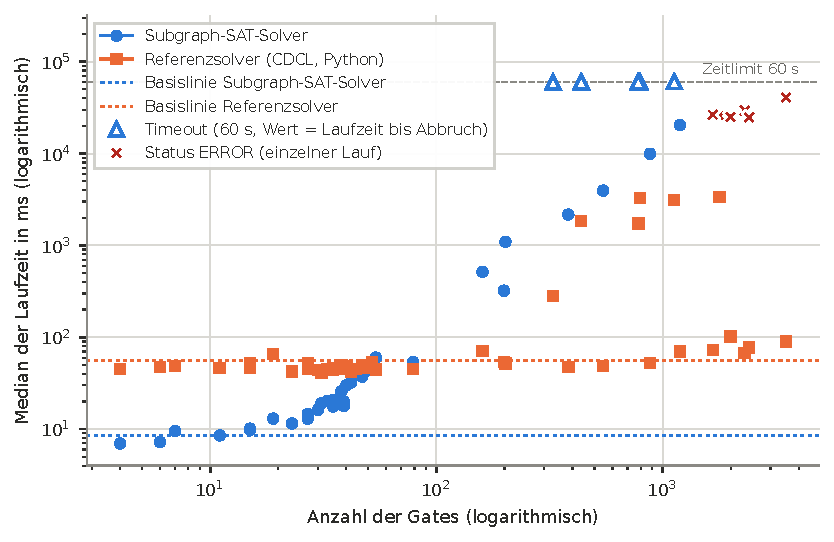
\includegraphics[width=\textwidth]{fig_v2_overview.pdf}
\caption{Median der Laufzeit aller 44 ausgewerteten Instanzen über der Gate-Anzahl (beide Achsen logarithmisch) für den Subgraph-SAT-Solver und den Referenzsolver der neuen Version 2.0.0.}
\label{fig:v2-overview}
\end{figure}

\paragraph{Aufbau der Abbildung.} Abbildung~\ref{fig:v2-overview} ist ein Streudiagramm mit logarithmischer Abszisse (Gate-Anzahl von $4$ bis $3\,512$) und logarithmischer Ordinate (Median in ms, von etwa $4$\,ms bis $3 \cdot 10^5$\,ms). Jede Instanz erscheint zweimal, einmal je Solver. Blaue Kreise sind Mediane des Subgraph-SAT-Solvers, orange Quadrate Mediane des Referenzsolvers. Weiße, blau umrandete Dreiecke markieren Instanzen, bei denen der Subgraph-SAT-Solver das Zeitlimit von $60$\,s erreichte; ihr Wert ist die Dauer des einen Laufs bis zum Abbruch ($60{,}04$ bis $60{,}27$\,s). Rote Kreuze markieren Instanzen mit dem Status \texttt{ERROR} (einzelner Lauf, Wert ist die Zeit bis zum Fehler). Die beiden gepunkteten horizontalen Linien sind die Basislinien ($8{,}43$\,ms blau, $56{,}18$\,ms orange), die gestrichelte graue Linie ist das Zeitlimit von $60$\,s. Da die Abszisse nur die Gate-Anzahl und nicht die Instanzfamilie kodiert, überlagern sich Punkte verschiedener Familien mit ähnlicher Gate-Anzahl.

\paragraph{Lesart: Subgraph-SAT-Solver.} Die blauen Punkte bilden drei Gruppen. Bei höchstens $79$ Gates (alle Target-AND-, Target-AND-Random-, c3-, c17- und die drei kleinen Miter-Instanzen) liegen sie zwischen $6{,}98$ und $60{,}04$\,ms, nahe der Basislinie und mit leichtem Anstieg zu größeren Instanzen. Ab etwa $160$ Gates steigen sie steil an: $515{,}75$\,ms bei c432 ($160$ Gates), $3\,945{,}39$\,ms bei c1355 ($546$ Gates), $20\,427{,}66$\,ms bei c2670 ($1\,193$ Gates), der größten gelösten Instanz. Bei einem Faktor $7{,}5$ in der Gate-Anzahl ($160$ bis $1\,193$) steigt die Laufzeit damit um den Faktor $39{,}6$. Die dritte Gruppe sind die fünf Dreiecke ($328$ bis $1\,125$ Gates, ausschließlich Miter-Instanzen) und die sechs Kreuze ($1\,669$ bis $3\,512$ Gates).

\paragraph{Lesart: Referenzsolver.} Die orangen Quadrate liegen für alle Nicht-Miter-Instanzen in einem flachen Band zwischen $41{,}02$ und $102{,}17$\,ms, in der Nähe der Basislinie von $56{,}18$\,ms, auch bei $3\,512$ Gates (c7552: $89{,}88$\,ms). Nur die sechs größeren Miter-Instanzen heben sich ab: Ihre Quadrate liegen zwischen $279{,}73$ und $3\,374{,}42$\,ms. Der Referenzsolver löst \emph{alle} 44 Instanzen, und seine Laufzeit liegt, mit Ausnahme dieser sechs Instanzen, im gesamten Bereich nahe an der Interpreter-Startzeit.

\paragraph{Kreuzung der Kurven.} Bei kleinen Instanzen (bis etwa $40$ Gates) liegt der Subgraph-SAT-Solver deutlich unter dem Referenzsolver, weil sein Prozessstart nur etwa $8$\,ms statt $56$\,ms kostet. Bei etwa $50$ Gates treffen sich die Kurven (Abschnitt~\ref{sec:v2-tiefe}); ab etwa $160$ Gates liegt der Subgraph-SAT-Solver deutlich darüber. Dieser Schnittpunkt ist vor allem ein Effekt der unterschiedlichen Startkosten der beiden Programme und keine Aussage über die Qualität der Algorithmen (Abschnitt~\ref{sec:v2-vergleich}).

\begin{figure}[ht]
\centering
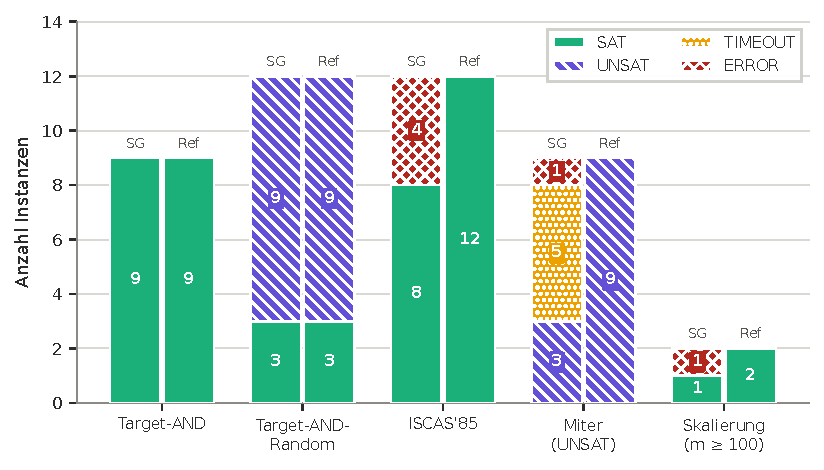
\includegraphics[width=0.92\textwidth]{fig_v2_status.pdf}
\caption{Anzahl der Instanzen je Instanzfamilie und Status (SAT, UNSAT, Timeout, ERROR) für den Subgraph-SAT-Solver (SG) und den Referenzsolver (Ref) der neuen Version 2.0.0.}
\label{fig:v2-status}
\end{figure}

\paragraph{Aufbau der Abbildung.} Abbildung~\ref{fig:v2-status} ist ein gestapeltes Balkendiagramm. Für jede der fünf Instanzfamilien (Target-AND, Target-AND-Random, ISCAS'85, Miter, Skalierung mit $m \ge 100$) stehen zwei Balken nebeneinander, links der Subgraph-SAT-Solver (SG), rechts der Referenzsolver (Ref). Die Höhe eines Balkens ist die Zahl der Instanzen der Familie, die Segmente zeigen die Anzahl je Status (grün: \texttt{SAT}, violett schraffiert: \texttt{UNSAT}, gelb gepunktet: Timeout, rot gekreuzt: \texttt{ERROR}); die Zahl im Segment ist die Instanzzahl.

\paragraph{Lesart.} Der Referenzsolver erreicht bei allen $44$ Instanzen ein Ergebnis: Target-AND $9\times$\,SAT, Target-AND-Random $3\times$\,SAT und $9\times$\,UNSAT, ISCAS'85 $12\times$\,SAT, Miter $9\times$\,UNSAT, Skalierung $2\times$\,SAT. Der Subgraph-SAT-Solver erreicht bei $33$ Instanzen ein Ergebnis, bei $5$ ein Timeout und bei $6$ den Status \texttt{ERROR}. Auf Target-AND und Target-AND-Random liefern beide Solver auf allen Instanzen dasselbe Ergebnis. Bei ISCAS'85 fallen $4$ von $12$ Instanzen (c3540, c5315, c6288, c7552) mit \texttt{ERROR} aus, bei den Miter-Instanzen sind es $5$ Timeouts und $1$ \texttt{ERROR}, bei den Skalierungsinstanzen ein \texttt{ERROR} (\texttt{TargetAND\_m1000}). Der Subgraph-SAT-Solver löst damit alle erfüllbaren Instanzen bis $1\,193$ Gates und die kleinen unerfüllbaren Instanzen; an allen sechs Instanzen ab $1\,669$ Gates scheitert er mit \texttt{ERROR}.

\subsubsection{Experiment 1: Target-AND und Skalierung}

Tabelle~\ref{tab:v2-target-and} zeigt Struktur, Status und Mediane für die neun Target-AND-Circuits mit $m=4,\ldots,20$ und die beiden ausgewerteten Skalierungsinstanzen ($m=100$ und $m=1000$). Abbildung~\ref{fig:v2-target-and} stellt sie grafisch dar.

\begin{table}[ht]
\centering\scriptsize
\setlength{\tabcolsep}{3.2pt}
\input{\resultsdir/paper/tab_v2_target_and.tex}
\caption{Target-AND und Skalierung: Struktur, Status (Subgraph-SAT-Solver / Referenzsolver, falls verschieden) und Median $\tilde{t}$ der Laufzeit in ms (SG: Subgraph-SAT-Solver, Ref: Referenzsolver; $n$: Zahl der Messläufe).}
\label{tab:v2-target-and}
\end{table}

\begin{figure}[ht]
\centering
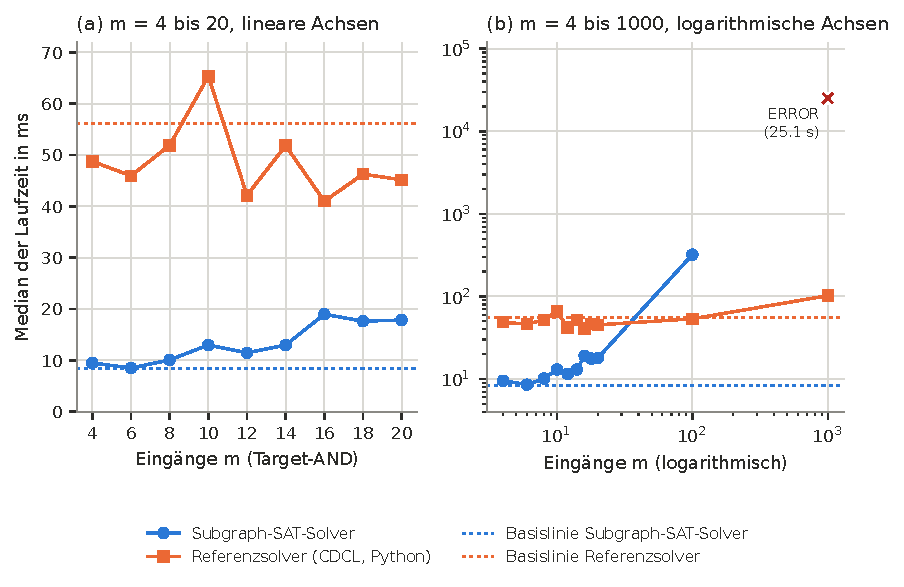
\includegraphics[width=\textwidth]{fig_v2_target_and.pdf}
\caption{Median der Laufzeit der Target-AND-Circuits in Abhängigkeit von der Eingangszahl $m$, links für $m=4$ bis $20$ (lineare Achsen), rechts bis $m=1000$ (logarithmische Achsen), für beide Solver.}
\label{fig:v2-target-and}
\end{figure}

\paragraph{Aufbau der Abbildung.} Abbildung~\ref{fig:v2-target-and} hat zwei Teilbilder. In Teilbild~(a) sind die neun Mediane für $m=4,6,\ldots,20$ auf linearen Achsen aufgetragen (Ordinate $0$ bis $72$\,ms), jeweils als Linienzug mit Punkten: blaue Kreise für den Subgraph-SAT-Solver, orange Quadrate für den Referenzsolver. Die gepunkteten Linien sind die Basislinien. Teilbild~(b) enthält dieselben Punkte und zusätzlich $m=100$ und $m=1000$ auf doppelt-logarithmischen Achsen (Abszisse $m$, Ordinate $4$ bis $1{,}2 \cdot 10^5$\,ms). Bei $m=1000$ endet der blaue Linienzug; dort steht ein rotes Kreuz mit der Beschriftung \glqq ERROR (25,1~s)\grqq{}, das den fehlgeschlagenen Lauf des Subgraph-SAT-Solvers kennzeichnet. Der orange Linienzug läuft bis $m=1000$ durch.

\paragraph{Lesart von Teilbild (a).} Der Median des Subgraph-SAT-Solvers steigt von $9{,}52$\,ms bei $m=4$ nicht streng monoton, aber erkennbar auf $17{,}88$\,ms bei $m=20$. Das Minimum liegt bei $m=6$ ($8{,}53$\,ms), das Maximum bei $m=16$ ($19{,}02$\,ms). Eine lineare Regression über die neun Werte ergibt eine Steigung von $0{,}66$\,ms je zusätzlichem Eingang bei $R^2 = 0{,}836$; die Rangkorrelation nach Spearman beträgt $\rho = 0{,}883$ ($n=9$). Der Anstieg ist klein gegen die Instanzgröße: Gates, Klauseln und Literale wachsen von $m=4$ bis $m=20$ um den Faktor $5{,}6$ ($7 \to 39$ Gates, $38 \to 214$ Literale), der Median aber nur um den Faktor $1{,}9$. Abzüglich der Basislinie ($8{,}43$\,ms) bleiben Nettozeiten zwischen $0{,}1$ und $10{,}6$\,ms; für $m \le 8$ liegen die Mediane höchstens $1{,}7$\,ms über der Basislinie und sind damit praktisch nicht von der Prozessstart-Grundlast zu unterscheiden. Der Median des Referenzsolvers dagegen zeigt keinen Anstieg: Er liegt zwischen $41{,}02$\,ms ($m=16$) und $65{,}36$\,ms ($m=10$), also um die Basislinie von $56{,}18$\,ms, und acht der neun Werte liegen darunter. Die Steigung beträgt $-0{,}41$\,ms je Eingang bei $R^2 = 0{,}093$ und $\rho = -0{,}417$. Der Referenzsolver misst in diesem Bereich somit praktisch nur den Interpreterstart; die Rechenzeit für die Formel geht im Rauschen des Prozessstarts unter.

\paragraph{Lesart von Teilbild (b).} Mit $m=100$ ($199$ Gates, $498$ Klauseln, $1\,094$ Literale) steigt der Median des Subgraph-SAT-Solvers auf $321{,}23$\,ms und liegt damit $6{,}0$-mal über dem des Referenzsolvers ($53{,}56$\,ms). Von $m=20$ ($17{,}88$\,ms, $214$ Literale) auf $m=100$ wächst die Laufzeit um den Faktor $18{,}0$ bei einem Literal-Faktor von $5{,}1$. Zieht man die Basislinie ab, ergibt sich ein Faktor $33{,}1$ und, auf die Literalzahl bezogen, ein Exponent von etwa $2{,}1$; das ist ein Wert in der Größenordnung des Exponenten, der in Abschnitt~\ref{sec:v2-iscas} aus den ISCAS-Messungen bestimmt wird, aber aus nur zwei Punkten gewonnen. Bei $m=1000$ ($1\,999$ Gates, $4\,998$ Klauseln, $10\,994$ Literale) scheitert der Subgraph-SAT-Solver mit \texttt{ERROR} nach $25{,}09$\,s; die Instanz ist aber nach Konstruktion erfüllbar (eindeutige Belegung), und der Referenzsolver löst sie mit $102{,}17$\,ms korrekt als \texttt{SAT}. Das Programm markiert diesen Lauf deshalb als \glqq unerwartetes Ergebnis\grqq{}. Der Referenzsolver wächst von $m=100$ auf $m=1000$ nur von $53{,}56$ auf $102{,}17$\,ms.

\subsubsection{Experiment 2: Target-AND-Random, Variation der Tiefe}
\label{sec:v2-tiefe}

Bei festem $m=10$ wächst der Circuit mit der Tiefe $d$ von $27$ Gates und $174$ Literalen ($d=1$) auf $54$ Gates und $409$ Literale ($d=12$); Tabelle~\ref{tab:v2-depth} und Abbildung~\ref{fig:v2-depth} zeigen die Ergebnisse.

\begin{table}[ht]
\centering\scriptsize
\setlength{\tabcolsep}{3.2pt}
\input{\resultsdir/paper/tab_v2_depth.tex}
\caption{Target-AND-Random ($m=10$): Struktur, Status und Median $\tilde{t}$ der Laufzeit in ms für beide Solver (Bezeichnungen wie in Tabelle~\ref{tab:v2-target-and}).}
\label{tab:v2-depth}
\end{table}

\begin{figure}[ht]
\centering
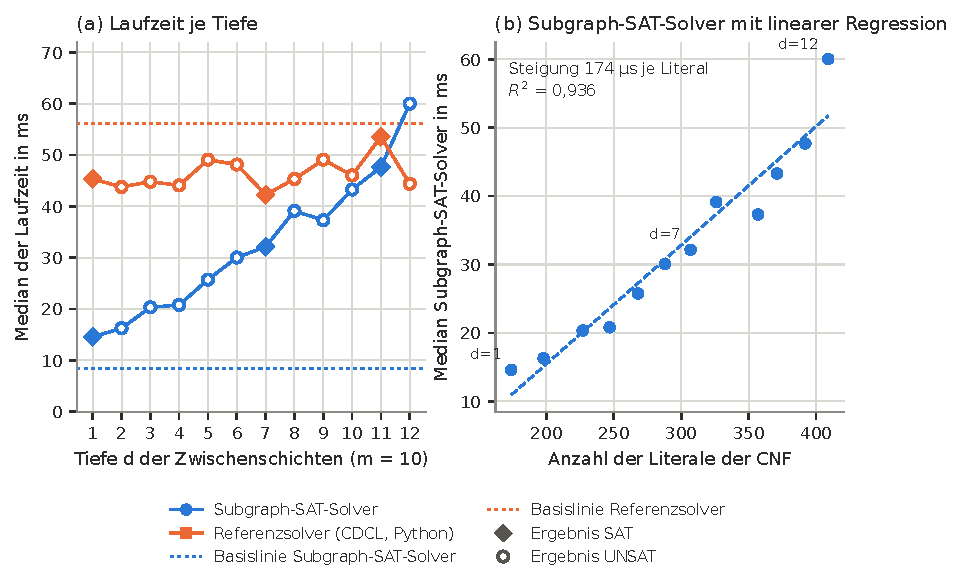
\includegraphics[width=\textwidth]{fig_v2_depth.pdf}
\caption{Median der Laufzeit der Target-AND-Random-Circuits ($m=10$) über der Tiefe $d$ für beide Solver mit Kennzeichnung von SAT und UNSAT (links) und über der Literalzahl mit linearer Regression für den Subgraph-SAT-Solver (rechts).}
\label{fig:v2-depth}
\end{figure}

\paragraph{Aufbau der Abbildung.} In Teilbild~(a) von Abbildung~\ref{fig:v2-depth} ist die Tiefe $d=1,\ldots,12$ auf der Abszisse und der Median in ms auf der Ordinate aufgetragen (Ordinate $0$ bis $72$\,ms). Der blaue Linienzug gehört zum Subgraph-SAT-Solver, der orange zum Referenzsolver. Die Form der Marker kodiert das Ergebnis: Gefüllte Rauten bedeuten \texttt{SAT} ($d=1,7,11$), weiße Kreise mit farbigem Rand bedeuten \texttt{UNSAT} (alle übrigen Tiefen). Beide Solver liefern bei jeder Tiefe dasselbe Ergebnis. Die gepunkteten Linien sind die Basislinien. Teilbild~(b) trägt für den Subgraph-SAT-Solver den Median über der Literalzahl der CNF ($174$ bis $409$) auf und zeigt die Regressionsgerade als gestrichelte Linie; im Bild sind die Steigung ($174$\,$\mu$s je Literal) und das Bestimmtheitsmaß ($R^2 = 0{,}936$) angegeben. Die Punkte für $d=1$, $d=7$ und $d=12$ sind beschriftet.

\paragraph{Lesart von Teilbild (a).} Der Median des Subgraph-SAT-Solvers steigt mit der Tiefe nahezu monoton von $14{,}59$\,ms ($d=1$) auf $60{,}04$\,ms ($d=12$), also um den Faktor $4{,}1$ bei einer Verdopplung der Gate-Zahl ($27 \to 54$) und einem Literal-Faktor von $2{,}35$. Es gibt genau eine Abweichung von der Monotonie: Bei $d=9$ ($37{,}32$\,ms) liegt der Median unter dem von $d=8$ ($39{,}13$\,ms). Die Spearman-Korrelation zwischen Tiefe und Median beträgt $\rho = 0{,}993$ ($n=12$), die lineare Regression ergibt $3{,}73$\,ms je Tiefenschicht bei $R^2 = 0{,}953$. Der Median des Referenzsolvers dagegen schwankt unsystematisch zwischen $42{,}28$\,ms ($d=7$) und $53{,}58$\,ms ($d=11$), die Steigung beträgt $0{,}33$\,ms je Schicht bei $R^2 = 0{,}145$ und $\rho = 0{,}343$. Er bleibt auf dem Niveau der Basislinie. Die Kurven kreuzen sich zwischen $d=11$ ($47{,}68$ gegenüber $53{,}58$\,ms) und $d=12$ ($60{,}04$ gegenüber $44{,}42$\,ms): Bei $d=12$ ist der Subgraph-SAT-Solver erstmals langsamer als der Referenzsolver ($1{,}35$-faches).

\paragraph{Lesart von Teilbild (b).} Die Punkte liegen eng an der Geraden mit der Steigung $0{,}174$\,ms je Literal. Die größten Abweichungen sind $+8{,}29$\,ms bei $d=12$, $-5{,}39$\,ms bei $d=9$, $+3{,}67$\,ms bei $d=1$ und $-2{,}78$\,ms bei $d=4$; alle übrigen Abweichungen betragen weniger als $2{,}0$\,ms. Das Verhältnis der Messwerte zur Geraden ist bei den \texttt{SAT}-Instanzen ($d=1,7,11$: $+3{,}67$, $-1{,}88$, $-1{,}11$\,ms) nicht anders als bei den \texttt{UNSAT}-Instanzen; in diesem Größenbereich ist also kein Unterschied zwischen erfüllbaren und unerfüllbaren Formeln erkennbar. Der Achsenabschnitt der Geraden ($-19{,}3$\,ms) ist negativ; die Gerade beschreibt deshalb nur den Bereich der Messpunkte ($174$ bis $409$ Literale) und nicht das Verhalten bei sehr kleinen Instanzen, wo die Basislinie dominiert. Bei den Selbst-Miter-Instanzen von Target-AND (\texttt{MiterSelf\_TargetAND\_m10}: $219$ Literale, \texttt{MiterSelf\_TargetAND\_m20}: $439$ Literale) liegen die Messwerte ($19{,}97$ und $53{,}58$\,ms) nahe an dem, was die Gerade für diese Literalzahlen ergibt ($18{,}7$ und $57{,}0$\,ms), obwohl es sich um andere, ebenfalls unerfüllbare Formeln handelt.

\subsubsection{Experiment 3: ISCAS'85}
\label{sec:v2-iscas}

Tabelle~\ref{tab:v2-iscas} und Abbildung~\ref{fig:v2-iscas} zeigen die zwölf ISCAS'85-Circuits mit $4$ bis $3\,512$ Gates ($26$ bis $21\,945$ Literale).

\begin{table}[ht]
\centering\scriptsize
\setlength{\tabcolsep}{3.2pt}
\input{\resultsdir/paper/tab_v2_iscas.tex}
\caption{ISCAS'85: Struktur, Status und Median $\tilde{t}$ der Laufzeit in ms für beide Solver, aufsteigend nach Gate-Anzahl (Bezeichnungen wie in Tabelle~\ref{tab:v2-target-and}).}
\label{tab:v2-iscas}
\end{table}

\begin{figure}[ht]
\centering
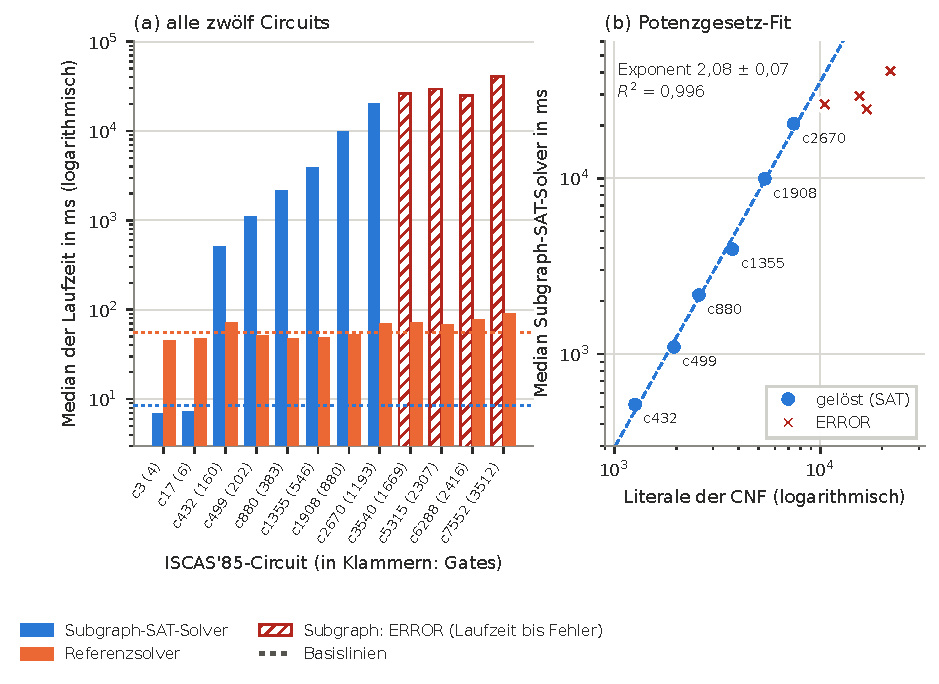
\includegraphics[width=\textwidth]{fig_v2_iscas.pdf}
\caption{Median der Laufzeit der zwölf ISCAS'85-Circuits für beide Solver (links) und Potenzgesetz-Fit des Subgraph-SAT-Solvers über der Literalzahl der CNF für die sechs gelösten Circuits von c432 bis c2670 (rechts).}
\label{fig:v2-iscas}
\end{figure}

\paragraph{Aufbau der Abbildung.} Teilbild~(a) von Abbildung~\ref{fig:v2-iscas} ist ein Balkendiagramm mit logarithmischer Ordinate (Median in ms, $3$ bis $10^5$). Die zwölf Circuits stehen in gleichen Abständen, aufsteigend nach Gate-Anzahl von c3 ($4$ Gates) bis c7552 ($3\,512$ Gates); die Abszisse ist daher kategorial, und die Gate-Anzahl steht in Klammern hinter dem Namen. Je Circuit gibt es zwei Balken: blau für den Subgraph-SAT-Solver, orange für den Referenzsolver. Rot schraffierte Balken mit weißer Füllung kennzeichnen \texttt{ERROR}-Läufe des Subgraph-SAT-Solvers; ihre Höhe ist die Zeit bis zum Fehler. Die gepunkteten Linien sind die Basislinien. Teilbild~(b) trägt die Mediane der sechs gelösten Circuits c432, c499, c880, c1355, c1908 und c2670 doppelt-logarithmisch über der Literalzahl der CNF ($1\,259$ bis $7\,422$) auf (blaue Punkte, beschriftet), dazu die angepasste Potenzfunktion als gestrichelte Gerade. Die Kreuze zeigen die vier fehlgeschlagenen Circuits (c3540 bis c7552) an ihrer Literalzahl; sie gehen nicht in den Fit ein. Ebenfalls nicht im Fit enthalten sind c3 und c17, deren Mediane ($6{,}98$ und $7{,}24$\,ms) unter der Basislinie liegen.

\paragraph{Lesart von Teilbild (a): Subgraph-SAT-Solver.} Die blauen Balken wachsen von links nach rechts über drei Größenordnungen: c3 und c17 liegen bei $6{,}98$ und $7{,}24$\,ms, c432 bei $515{,}75$\,ms, c499 bei $1\,094{,}34$\,ms, c880 bei $2\,167{,}29$\,ms, c1355 bei $3\,945{,}39$\,ms, c1908 bei $9\,931{,}22$\,ms und c2670 bei $20\,427{,}66$\,ms. Dieses Wachstum ist durchgehend monoton. Die Zahl der Wiederholungen sinkt dabei mit der Laufzeit durch das Zeitbudget: $n=30$ bis c880, $n=13$ bei c1355, $n=6$ bei c1908 und $n=3$ bei c2670. Die Mediane der drei größten gelösten Circuits stützen sich also auf wenige Läufe. Die vier Circuits ab $1\,669$ Gates (c3540, c5315, c6288, c7552) enden mit \texttt{ERROR} nach $26{,}36$, $29{,}42$, $24{,}77$ und $40{,}74$\,s (je ein Lauf, da bereits der Warm-up fehlschlug). Diese Zeiten sind keine Lösungszeiten.

\paragraph{Lesart von Teilbild (a): Referenzsolver.} Die orangen Balken sind flach: von $45{,}19$\,ms (c3) bis $89{,}88$\,ms (c7552), der Median dieser zwölf Werte beträgt $60{,}17$\,ms, nahe der Basislinie. Der Referenzsolver findet für alle zwölf Circuits (mit Ausgang auf wahr) eine erfüllende Belegung. Eine leichte Zunahme mit der Größe ist erkennbar (die vier größten Circuits stehen mit $67{,}58$ bis $89{,}88$\,ms am oberen Ende), sie beträgt aber nur wenige Dutzend Millisekunden.

\paragraph{Lesart von Teilbild (b).} Die sechs Punkte liegen nahezu auf einer Geraden. Die Anpassung $t \propto L^{b}$ mit der Literalzahl $L$ ergibt einen Exponenten $b = 2{,}08$ mit einem Standardfehler von $0{,}07$ und $R^2 = 0{,}996$. Das $95$\,\%-Konfidenzintervall der Steigung ($t$-Verteilung mit $4$ Freiheitsgraden) beträgt rund $[1{,}89;\ 2{,}27]$. Der Exponent liegt damit in der Nähe von $2$. Das ist mit der in Abschnitt~\ref{sec:solver-impl} beschriebenen Struktur vereinbar, in der die Adjazenzmatrix des Clique-Graphen durch paarweise Vergleiche der Literalvorkommen aufgebaut wird und $O(L^2)$ Schritte benötigt; bewiesen ist dieser Zusammenhang durch die Messung aber nicht. Der Fit stützt sich auf nur sechs Punkte aus verschiedenen Circuits (nicht auf eine Instanzfamilie mit einem Parameter) und auf Mediane, die bei c1355, c1908 und c2670 aus $13$, $6$ und $3$ Läufen stammen. Er gilt außerdem nur für die gemessene Literalzahl der CNF und nicht für die tatsächliche Knotenzahl des Clique-Graphen (nach der Normalisierung auf höchstens drei Literale je Klausel sind Letztere etwas größer). Die Rechenzeit des externen Subgraph-Prozesses ist in diesem Wert nicht von der Reduktion getrennt (Abschnitt~\ref{sec:solver-impl}). Insbesondere liefert der Fit keine Bestätigung oder Widerlegung der theoretischen Schranke $\Theta(n^3)$ des Subgraph Algorithmus.

\paragraph{Der Ausfall ab $10\,487$ Literalen.} Alle ISCAS-Circuits bis $7\,422$ Literale (c2670) werden gelöst; alle ab $10\,487$ Literalen (c3540) enden mit \texttt{ERROR}. Dieselbe Trennung zeigt der gesamte Datensatz: Alle sechs Instanzen mit \texttt{ERROR} haben mindestens $10\,487$ Literale ($10\,487$, $10\,994$, $11\,125$, $15\,466$, $16\,817$ und $21\,945$), alle Instanzen mit höchstens $7\,958$ Literalen enden mit einem Ergebnis oder einem Timeout. Insbesondere fällt auch \texttt{TargetAND\_m1000} aus, ein einfacher AND-Baum, den der Referenzsolver in $102$\,ms löst. Der Ausfall hängt also an der Instanzgröße und nicht an der logischen Schwierigkeit der Formel. Die Fehlerzeiten ($24{,}77$ bis $40{,}74$\,s) liegen deutlich unter dem Zeitlimit von $60$\,s; die Läufe endeten also nicht durch das Zeitlimit. Die Ursache wurde nicht untersucht. Die CSV-Datei des Zwischenstands enthält weder Rückgabecode noch Fehlermeldung (Abschnitt~\ref{sec:v2-daten}). Zu prüfen wären unter anderem der Speicherbedarf der Reduktion und des externen Subgraph-Prozesses auf der Maschine mit $3{,}9$\,GiB ohne Swap, die Größe der JSON-Dateien mit den Kantenlisten sowie eine interne Fehlerbehandlung des Solvers (Abschnitt~\ref{sec:v2-hardware}). Dass der Lauf des Full-Presets bei \texttt{TargetAND\_m10000} ($109\,994$ Literale) abbrach, passt zu dieser Größenschwelle, ist aber nicht belegt.

\subsubsection{Miter-Instanzen: unerfüllbare Formeln}

Die neun Miter-Instanzen sind unerfüllbar. Tabelle~\ref{tab:v2-miter} und Abbildung~\ref{fig:v2-miter} zeigen die Ergebnisse.

\begin{table}[ht]
\centering\scriptsize
\setlength{\tabcolsep}{3.2pt}
\input{\resultsdir/paper/tab_v2_miter.tex}
\caption{Miter-Instanzen (alle unerfüllbar): Struktur, Status und Median $\tilde{t}$ der Laufzeit in ms für beide Solver, aufsteigend nach Gate-Anzahl (Bezeichnungen wie in Tabelle~\ref{tab:v2-target-and}).}
\label{tab:v2-miter}
\end{table}

\begin{figure}[ht]
\centering
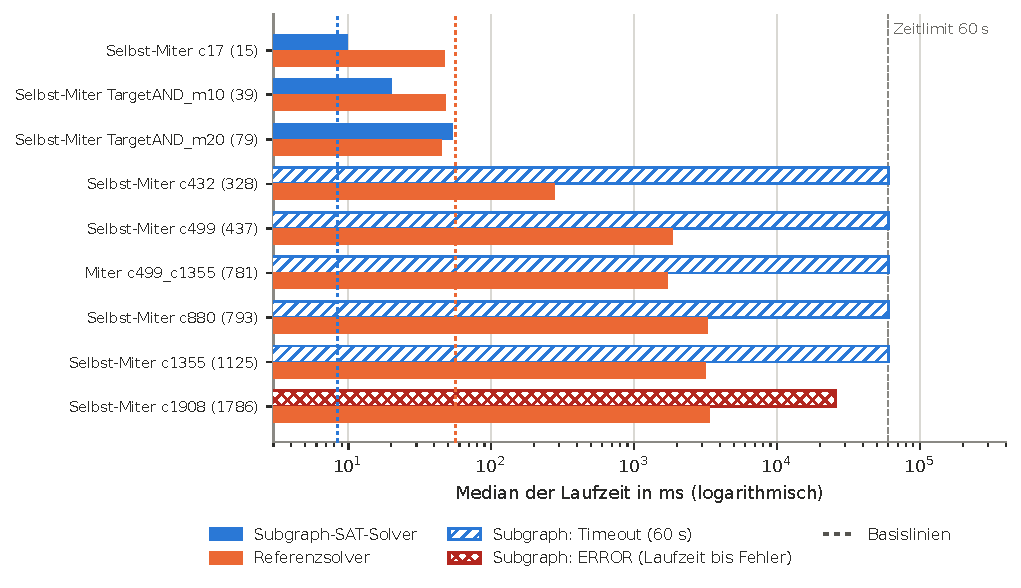
\includegraphics[width=\textwidth]{fig_v2_miter.pdf}
\caption{Median der Laufzeit der neun unerfüllbaren Miter-Instanzen für beide Solver mit Kennzeichnung der Timeouts und des ERROR-Laufs des Subgraph-SAT-Solvers.}
\label{fig:v2-miter}
\end{figure}

\paragraph{Aufbau der Abbildung.} Abbildung~\ref{fig:v2-miter} ist ein horizontales, gruppiertes Balkendiagramm mit logarithmischer Abszisse (Median in ms, von $3$ bis $4 \cdot 10^5$). Jede Instanz hat eine Zeile mit zwei Balken, oben blau für den Subgraph-SAT-Solver, unten orange für den Referenzsolver. Die Zeilen sind aufsteigend nach Gate-Anzahl (in Klammern) sortiert, die kleinste oben. Blau schraffierte Balken mit weißer Füllung kennzeichnen Timeouts des Subgraph-SAT-Solvers; sie enden bei etwa $60$\,s, der senkrechten gestrichelten Linie. Der rot gekreuzte Balken der untersten Zeile ist der \texttt{ERROR}-Lauf bei \texttt{MiterSelf\_c1908}. Die beiden gepunkteten senkrechten Linien sind die Basislinien.

\paragraph{Lesart.} Der Subgraph-SAT-Solver löst nur die drei kleinsten Instanzen: \path{MiterSelf_c17} ($15$ Gates, $9{,}86$\,ms), \path{MiterSelf_TargetAND_m10} ($39$ Gates, $19{,}97$\,ms) und \path{MiterSelf_TargetAND_m20} ($79$ Gates, $53{,}58$\,ms), jeweils korrekt als \texttt{UNSAT}. Alle anderen sechs Instanzen scheitern: Fünf laufen in das Zeitlimit (\path{MiterSelf_c432}, \path{MiterSelf_c499}, \path{Miter_c499_c1355}, \path{MiterSelf_c880}, \path{MiterSelf_c1355}; Dauer des einen Laufs $60\,041$ bis $60\,274$\,ms), und \path{MiterSelf_c1908} endet nach $25{,}56$\,s mit \texttt{ERROR} (nach Abschnitt~\ref{sec:v2-iscas} ist dies wegen der Größe von $11\,125$ Literalen zu erwarten). Der Referenzsolver löst dagegen \emph{alle neun} Instanzen korrekt als \texttt{UNSAT}: $46{,}92$, $47{,}66$ und $44{,}95$\,ms für die drei kleinsten (auf Höhe der Basislinie), dann $279{,}73$\,ms (c432), $1\,853{,}19$\,ms (c499), $1\,723{,}69$\,ms (c499 gegen c1355), $3\,293{,}14$\,ms (c880), $3\,139{,}56$\,ms (c1355) und $3\,374{,}42$\,ms (c1908). Die Mediane der größeren Miter-Instanzen sind nicht streng nach Gate-Anzahl geordnet: c880 mit $793$ Gates ($3{,}29$\,s) ist langsamer als c1355 mit $1\,125$ Gates ($3{,}14$\,s). Wegen des Zeitbudgets stützen sich diese Mediane auf unterschiedlich viele Läufe ($n=30$ bei c432 und c499, $19$ bei c880, $16$ bei c499 gegen c1355, $15$ bei c1908 und $7$ bei c1355).

\paragraph{Vergleich mit den erfüllbaren ISCAS-Instanzen.} Beim Subgraph-SAT-Solver ist der Unterschied zwischen erfüllbaren und unerfüllbaren Instanzen bei vergleichbarer Literalzahl groß: \texttt{MiterSelf\_c432} ($2\,623$ Literale) erreicht das Zeitlimit von $60$\,s, während die erfüllbare Instanz c880 mit $2\,571$ Literalen nach $2{,}17$\,s gelöst wird, also mindestens $27{,}7$-mal schneller. Ebenso liegen die übrigen vier Timeouts bei $4\,374$ bis $7\,958$ Literalen, wo c1355 ($3\,739$ Literale), c1908 ($5\,375$) und c2670 ($7\,422$) noch in $3{,}9$ bis $20{,}4$\,s gelöst werden. Aus diesen Daten allein lässt sich allerdings nicht entscheiden, ob dies an der Unerfüllbarkeit liegt oder an der Struktur der Miter-Formeln (die Miter-Formeln von c499, c880, c1355 und c1908 enthalten Klauseln mit $26$ bis $33$ Literalen, die ISCAS-Formeln höchstens $10$; \texttt{MiterSelf\_c432} hat wie c432 höchstens $10$), denn beides ändert sich gleichzeitig. Bei den kleinen unerfüllbaren Instanzen (Target-AND-Random mit $d \ge 2$, Selbst-Miter von Target-AND) gibt es keine Auffälligkeit (Abschnitt~\ref{sec:v2-tiefe}).

\subsubsection{Vergleich der beiden Solver}
\label{sec:v2-vergleich}

Abbildung~\ref{fig:v2-ratio} fasst das Verhältnis der Mediane beider Solver zusammen.

\begin{figure}[ht]
\centering
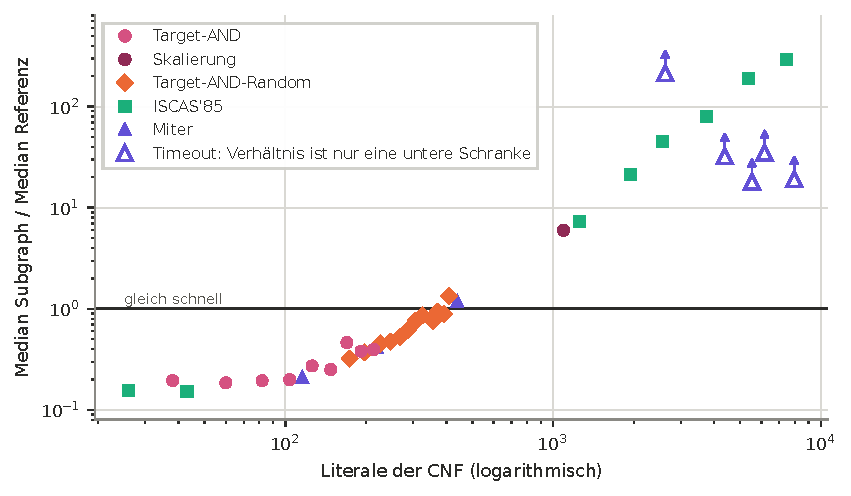
\includegraphics[width=\textwidth]{fig_v2_ratio.pdf}
\caption{Verhältnis des Medians des Subgraph-SAT-Solvers zum Median des Referenzsolvers je Instanz über der Literalzahl der CNF (beide Achsen logarithmisch), farbig nach Instanzfamilie.}
\label{fig:v2-ratio}
\end{figure}

\paragraph{Aufbau der Abbildung.} Abbildung~\ref{fig:v2-ratio} ist ein doppelt-logarithmisches Streudiagramm. Die Abszisse ist die Literalzahl der CNF ($26$ bis $21\,945$), die Ordinate der Quotient $\tilde{t}_{\mathrm{SG}} / \tilde{t}_{\mathrm{Ref}}$ der beiden Mediane. Die schwarze waagerechte Linie bei $1$ markiert Gleichstand; Punkte darunter bedeuten, dass der Subgraph-SAT-Solver schneller war. Die Farbe und Form der Marker kodiert die Instanzfamilie: magentafarbene Kreise für Target-AND (dunkles Magenta für die Skalierungsinstanz $m=100$), orange Rauten für Target-AND-Random, grüne Quadrate für ISCAS'85 und violette Dreiecke für Miter. Weiße Dreiecke mit Aufwärtspfeil sind Timeouts des Subgraph-SAT-Solvers; da der Lauf abgebrochen wurde, ist das gezeigte Verhältnis nur eine \emph{untere} Schranke des wahren Verhältnisses. Die sechs \texttt{ERROR}-Instanzen sind nicht eingezeichnet, weil ihr Median keine Lösungszeit ist.

\paragraph{Lesart.} Die Punkte steigen mit der Literalzahl von links unten nach rechts oben, weil der Referenzsolver kaum wächst (Abbildung~\ref{fig:v2-overview}), der Subgraph-SAT-Solver aber stark. Bei den $24$ Instanzen mit höchstens $392$ Literalen ist der Subgraph-SAT-Solver jeweils schneller (Quotient zwischen $0{,}15$ bei c3 und c17 und $0{,}94$ bei $d=10$); ab $409$ Literalen ($d=12$: $1{,}35$) ist er in allen Fällen langsamer: $1{,}19$ bei \texttt{MiterSelf\_TargetAND\_m20}, $6{,}0$ bei $m=100$, $7{,}2$ bei c432, $21{,}2$ bei c499, $45{,}5$ bei c880, $80{,}8$ bei c1355, $188{,}2$ bei c1908 und $291{,}5$ bei c2670, dem größten gelösten Verhältnis. Die Timeouts liegen bei Quotienten von mindestens $18{,}3$ bis mindestens $214{,}6$. Die Kreuzung bei rund $400$ Literalen ist vor allem ein Effekt der Startkosten ($8{,}43$\,ms gegenüber $56{,}18$\,ms). Sie hängt daher an der Wahl eines Python-Programms als Referenz und besagt nicht, dass der Subgraph-SAT-Solver für kleine Formeln einen besseren Algorithmus hat.

\subsubsection{Korrektheit und Übereinstimmung der Solver}

Bei $33$ Instanzen liefern beide Solver ein Ergebnis (\texttt{SAT} oder \texttt{UNSAT}); in allen $33$ Fällen sind die Ergebnisse gleich. Dies sind alle $9$ Target-AND-Circuits, alle $12$ Target-AND-Random-Circuits, $8$ ISCAS-Circuits (c3, c17, c432, c499, c880, c1355, c1908, c2670), die drei kleinen Miter-Instanzen und \texttt{TargetAND\_m100}. Bei den $13$ Instanzen dieser Menge, deren Ergebnis aus der Konstruktion folgt (Target-AND und \texttt{TargetAND\_m100}: \texttt{SAT}; Miter: \texttt{UNSAT}), stimmen beide Solver mit der erwarteten Antwort überein. Der Referenzsolver trifft die erwartete Antwort bei allen $20$ Instanzen mit bekanntem Ergebnis (Target-AND, Skalierung und Miter). Der Subgraph-SAT-Solver verfehlt sie bei zwei Instanzen, \texttt{MiterSelf\_c1908} und \texttt{TargetAND\_m1000}, jeweils mit \texttt{ERROR}; die Konsolenausgabe markiert beide als \glqq unerwartetes Ergebnis\grqq. Ein \texttt{ERROR} ist keine falsche Antwort, aber auch kein Ergebnis. Die Konsolenausgabe enthält keine Markierung \glqq Modell ungültig\grqq; für keine der ausgewerteten Instanzen wurde also gemeldet, dass ein ausgegebenes Modell die CNF oder den Circuit verletzt. Da die Modellprüfung nur für den ersten Lauf je Instanz und nur bei ausgegebenem Modell erfolgt und die Einzelergebnisse im Zwischenstand fehlen, kann dies nicht aus der CSV-Datei nachgeprüft werden.

%---------------------------------------------------------------------
\subsection{Diskussion der neuen Version}
\label{sec:v2-diskussion}

\subsubsection{Was die neuen Daten stützen}

\begin{itemize}
	\item \textbf{Die Messung enthält jetzt Skalierungsinformation.} Anders als in der ersten Messreihe, deren Werte für Instanzen von $4$ bis $3\,512$ Gates gleich blieben, wächst der Median des Subgraph-SAT-Solvers deutlich mit der Instanzgröße: bei Target-AND-Random um den Faktor $4{,}1$ zwischen $27$ und $54$ Gates, bei ISCAS'85 um mehr als drei Größenordnungen zwischen c17 und c2670. Die Basislinie von $8{,}43$\,ms ist so klein, dass Laufzeiten ab etwa $20$\,ms nicht mehr von ihr dominiert werden.
	\item \textbf{Näherungsweise quadratisches Wachstum im gemessenen Bereich.} Für die sechs gelösten ISCAS-Circuits von $1\,259$ bis $7\,422$ Literalen ergibt sich ein Exponent von $2{,}08 \pm 0{,}07$ (Standardfehler) über der Literalzahl.
	\item \textbf{Die Ergebnisse sind korrekt, soweit sie vorliegen.} In allen $33$ Fällen, in denen beide Solver entscheiden, stimmen sie überein, und alle bekannten erwarteten Antworten werden getroffen.
	\item \textbf{Kein sichtbarer Unterschied zwischen SAT und UNSAT bei kleinen Instanzen.} Bei Target-AND-Random liegen \texttt{SAT}- und \texttt{UNSAT}-Instanzen auf derselben Regressionsgeraden.
\end{itemize}

\subsubsection{Was die neuen Daten nicht stützen}

\begin{itemize}
	\item \textbf{Keine Aussage über die Schranke $\Theta(n^3)$.} Der Exponent $2{,}08$ gilt für die Literalzahl der CNF und für die gesamte Pipeline (Reduktion, Datei-I/O, externer Prozess), nicht für den Subgraph Algorithmus allein (Abschnitt~\ref{sec:solver-impl}). Er stützt sich auf sechs Punkte und bei den größten drei auf $13$, $6$ und $3$ Läufe.
	\item \textbf{Keine Aussage über etablierte SAT-Solver.} Der Referenzsolver ist ein Python-Programm ohne Anspruch auf Geschwindigkeit; sein Quotient zum Subgraph-SAT-Solver (Abbildung~\ref{fig:v2-ratio}) ist kein Maß für den Vergleich mit MiniSat oder CaDiCaL. Ein Vergleich mit diesen Solvern fehlt weiterhin.
	\item \textbf{Keine Aussage über die Ursache der \texttt{ERROR}-Läufe und der Timeouts.} Rückgabecode, Fehlermeldung und Speichernutzung liegen im Zwischenstand nicht vor. Dass die Ausfälle an der Instanzgröße hängen (ab $10\,487$ Literalen), ist ein Befund der Daten; warum sie auftreten, ist offen. Dass unerfüllbare Instanzen für den Subgraph-SAT-Solver schwerer sind, lässt sich aus den Daten nicht von der Wirkung der langen Klauseln der Miter trennen.
	\item \textbf{Keine Aussagen über die Streuung.} Es liegen nur Mediane vor. Konfidenzintervalle, Quartile und die Einzelläufe sind nicht verfügbar. Unterschiede von wenigen Millisekunden zwischen zwei Instanzen, etwa die Nicht-Monotonie bei $d=8$ und $d=9$, lassen sich deshalb nicht von Messrauschen unterscheiden.
	\item \textbf{Keine Skalierung bis $10^5$ Gates.} Die Skalierungsinstanzen $m=10\,000$ und $m=50\,000$ wurden nicht ausgewertet. Die größte gelöste Instanz hat $1\,193$ Gates.
\end{itemize}

\subsubsection{Gültigkeitsbedrohungen}

\begin{itemize}
	\item \textbf{Interne Validität.} Ein Kern teilt sich zwischen Solver und Messprozess. Die Basislinie des Referenzsolvers hat eine Standardabweichung von $14{,}63$\,ms bei einem Median von $56{,}18$\,ms; die Mediane des Referenzsolvers unter etwa $70$\,ms sind deshalb nicht voneinander zu unterscheiden. Die Basislinie wurde nur einmal vor dem Preset gemessen, nicht laufend.
	\item \textbf{Konstruktvalidität.} Gemessen wird die Wallclock-Zeit eines Prozesses einschließlich Prozessstart. Die solverinterne Zeit wird im Zwischenstand nicht berichtet. Die Spalte \texttt{runtime\_net\_ms} (Laufzeit minus Basislinie je Lauf) liegt im Zwischenstand nicht vor; Nettozeiten in diesem Abschnitt sind Differenzen von Medianen.
	\item \textbf{Externe Validität.} Die Target-AND-Instanzen sind einfache AND-Bäume mit eindeutiger Belegung; die Target-AND-Random-Instanzen sind klein ($27$ bis $54$ Gates). Industrielle Instanzen sind nur die ISCAS'85-Circuits mit bis zu $3\,512$ Gates; sie sind für moderne SAT-Solver klein. Die Ausgangsbedingung betrifft jeweils nur den ersten Ausgang.
	\item \textbf{Umgebung.} Eine virtuelle Maschine mit einer CPU, $3{,}9$\,GiB Speicher ohne Swap, Build ohne \texttt{-march=native} (Abschnitt~\ref{sec:v2-hardware}). Die Ergebnisse gelten für diese Umgebung; schon der Speicher kann die Grenze von $10\,487$ Literalen bestimmen.
	\item \textbf{Unvollständiger Lauf.} Der Full-Preset wurde nicht abgeschlossen (Abschnitt~\ref{sec:v2-daten}). Die ausgewerteten $44$ Instanzen sind vollständig, aber der Datensatz ist ein Zwischenstand.
\end{itemize}

\subsubsection{Vergleich der Befunde mit der ersten Messreihe}
\label{sec:v2-vergleich-erste}

Die Diskussion der ersten Messreihe hatte vermutet, dass deren konstante Laufzeiten ein Messartefakt aus Prozessstart und Zeitauflösung seien (Abschnitt~\ref{sec:diskussion}). Die neue Version stützt diese Vermutung in drei Punkten: (i) Mit nanosekundengenauer Zeitmessung liegen die Mediane nicht mehr auf den Zeittakten bei $15{,}625$ und $31{,}25$\,ms (die Einzelläufe sind im Zwischenstand nicht verfügbar). (ii) Die Basislinie der trivialen Instanz liegt mit $8{,}43$\,ms in der Größenordnung der kleinsten Messwerte kleiner Instanzen, und erst oberhalb davon steigen die Mediane mit der Instanzgröße. (iii) Bei größeren Instanzen wächst die Laufzeit des Subgraph-SAT-Solvers deutlich. Die in der ersten Messreihe beobachtete Unabhängigkeit der Laufzeit von der Instanzgröße war demnach keine Eigenschaft des Solvers. Der absolute Vergleich ist wegen der unterschiedlichen Instanzen (korrigierte Kodierung, Ausgangsbedingung) und der nicht dokumentierten Umgebung der ersten Messreihe nicht möglich (Abschnitt~\ref{sec:v2-einordnung}).

Die erste Messreihe fand außerdem keine Solver-Ausgabe. Die neue Version zeigt, dass der Subgraph-SAT-Solver bei den kleinen und mittleren Instanzen ein Ergebnis liefert, das mit dem Referenzsolver übereinstimmt.

\subsubsection{Offene Punkte}

\begin{enumerate}
	\item Den Full-Preset vollständig wiederholen und dabei \texttt{experiment\_results.csv}, \texttt{summary.csv}, \texttt{environment.json}, \texttt{baseline.json} und Rückgabecodes sichern; insbesondere klären, warum der Lauf bei \texttt{TargetAND\_m10000} abbrach.
	\item Die Ursache der \texttt{ERROR}-Läufe ab $10\,487$ Literalen untersuchen (Rückgabecode, Fehlermeldung, Speichernutzung \texttt{peak\_memory\_mb}) und die Skalierungsinstanzen $m=10\,000$ und $m=50\,000$ auf einer Maschine mit mehr Speicher messen.
	\item Den Solver mit CMake (\texttt{-O3 -march=native}) bauen und messen; die Version des Solvers festhalten.
	\item Den Referenzsolver durch MiniSat oder CaDiCaL ergänzen, damit der Vergleich nicht mehr durch die Startzeit des Python-Interpreters bestimmt wird.
	\item Mehr Messpunkte zwischen $1\,000$ und $10\,000$ Literalen (z.\,B.\ Target-AND mit $m=200$ bis $800$), um den Exponenten an einer Instanzfamilie mit einem Parameter zu prüfen, und Instanzen mit gleicher Literalzahl, aber unterschiedlicher Klausellänge, um den Einfluss der Klauseln der Miter von dem der Unerfüllbarkeit zu trennen.
\end{enumerate}

%---------------------------------------------------------------------
\subsection{Reproduktion der neuen Auswertung}
\label{sec:v2-repro}

Die Rohdaten des Zwischenstands liegen unter \path{src/results/}:

\begin{lstlisting}[language=bash, caption=Dateien der neuen Version 2.0.0 (Zwischenstand)]
src/results/
  full_zwischenstand.csv       Median je Solver und Instanz (88 Zeilen)
  full_log_zwischenstand.log   Konsolenausgabe des Full-Laufs (mit Basislinien)
  hardware.md                  Hardware und Software der Messungen
  paper/                       fig_v2_*.pdf, tab_v2_*.tex, summary_v2.json
\end{lstlisting}

Die Abbildungen und Tabellen dieses Abschnitts erzeugt das Skript \path{src/paper_analysis_v2.py}:

\begin{lstlisting}[language=bash, caption=Erzeugung der Auswertung der neuen Version]
pip install -e .
python -m src.paper_analysis_v2
cd science && pdflatex subgraph-sat-solver-experiments.tex
\end{lstlisting}

Das Skript berechnet die Struktur der Instanzen (Variablen, Klauseln, Literale) mit den Generatoren des Frameworks neu, prüft sie gegen die gemessenen Gate-Zahlen und schreibt alle im Text genannten Kennzahlen (Regressionen, Korrelationen, Exponent, Statuszähler) nach \path{src/results/paper/summary_v2.json}. Ein vollständiger neuer Lauf wird mit \path{python -m src.run_experiments --preset full --solver-path <Pfad> --with-reference} gestartet.

%=====================================================================
\section{Zusammenfassung}

Wir haben alle 288 Läufe der vier Experiment-Suites des Subgraph-SAT-Solver-Frameworks ausgewertet. Die Laufzeiten liegen zwischen $6{,}02$ und $40{,}27$\,ms und sind über Instanzgrößen von $4$ bis $3\,512$ Gates, über alle drei Circuit-Typen und über alle vier Suites statistisch nicht unterscheidbar. Ein Zusammenhang mit Gate-Anzahl ($\rho = 0{,}024$), Tiefe ($\rho = -0{,}086$) oder Eingangszahl liegt nicht vor. Die Messwerte häufen sich bei $15{,}625$ und $31{,}25$\,ms, und in keinem Lauf wurde ein Solver-Ergebnis erfasst. Zudem kodiert der CNF-Encoder die Gate-Typen NAND, NOR und XOR fehlerhaft, was die ISCAS'85-Formeln betrifft. Die Messungen sind daher als Obergrenze für die Prozesslaufzeit zu lesen (der Solver-Prozess endet für alle Instanzen ohne Timeout in unter $41$\,ms), nicht als Skalierungsstudie und nicht als Nachweis korrekter Lösungen. Die in Abschnitt~\ref{sec:diskussion} beschriebenen Änderungen am Messaufbau sind Voraussetzung dafür, das Skalierungsverhalten des Solvers und die theoretische $\Theta(n^3)$-Schranke empirisch zu prüfen.

\subsection{Ausblick}

\begin{itemize}
	\item Wiederholung aller Experimente mit dem verbesserten Messaufbau.
	\item Analyse von Strukturmaßen der ISCAS-Instanzen (Tiefe, Fan-out, Clustering) und ihres Einflusses auf die Solver-Zeit.
	\item Untersuchung unerfüllbarer Instanzen sowie Worst-Case-Konstruktionen für den Subgraph Algorithmus.
	\item Vergleich mit klassischen SAT-Solvern auf identischen Eingaben.
\end{itemize}

\subsection{Implementierungshinweis}

Der Code und die Rohdaten sind verfügbar unter: \url{https://github.com/naphez86/subgraph-sat-solver-experiments}.

%=====================================================================
\appendix

\section{Reproduzierbarkeit und Datenquellen}
\label{sec:repro}

Alle Rohdaten liegen unter \texttt{src/results/<suite>/}:

\begin{lstlisting}[language=bash, caption=Ergebnisstruktur]
src/results/
  quick/        experiment_results.{json,csv}   21 Laeufe
  standard/     experiment_results.{json,csv}   33 Laeufe
  full/         experiment_results.{json,csv}  117 Laeufe
  performance/  experiment_results.{json,csv}  117 Laeufe
  paper/        Tabellen (.tex), Abbildungen (.pdf), summary.json
\end{lstlisting}

Tabellen und Abbildungen dieser Arbeit werden aus den CSV-Dateien erzeugt:

\begin{lstlisting}[language=bash, caption=Erzeugung der Auswertung]
pip install -e ".[paper]"
python -m src.paper_analysis
cd science && pdflatex subgraph-sat-solver-experiments.tex
\end{lstlisting}

Das Skript schreibt nach \texttt{src/results/paper/}; die Kennzahlen im Text (Korrelationen, Testwerte, Anteile) sind zusätzlich in \texttt{summary.json} abgelegt.

\section{Beispiel-Datensätze}

Die folgenden Zeilen stammen unverändert aus \url{src/results/full/experiment_results.csv} (Spalten gekürzt):

\begin{lstlisting}[caption=Ausgewaehlte Datensaetze der Full-Suite]
circuit_type,circuit_name,num_inputs,num_gates,num_clauses,satisfiable,runtime_ms,timestamp
target_and,TargetAND_m4,4,7,20,False,22.2797,2026-07-14 09:40:24
target_and_random,TargetAND_m10_d1,10,27,91,False,15.6600,2026-07-14 09:40:24
iscas85,c7552,207,3512,10690,False,15.7025,2026-07-14 09:40:27
\end{lstlisting}

\section{Diagramme der einzelnen Suites}

Das Framework erzeugt für jede Suite sechs Diagramme (Laufzeit gegen Größe, Verteilung, Gates gegen Laufzeit, Klausel-Histogramm, Leistungsvergleich, Skalierungsanalyse) als SVG und PDF unter \texttt{src/results/<suite>/plots/}. Abbildung~\ref{fig:suiteplots} zeigt exemplarisch das Streudiagramm \glqq Gates gegen Laufzeit\grqq{} aller vier Suites; die Abbildungen der anderen Diagrammtypen und die zugehörigen Textberichte (\texttt{report.txt}) liegen im selben Ordner.

\begin{figure}[H]
\centering
\begin{subfigure}[b]{0.48\textwidth}
	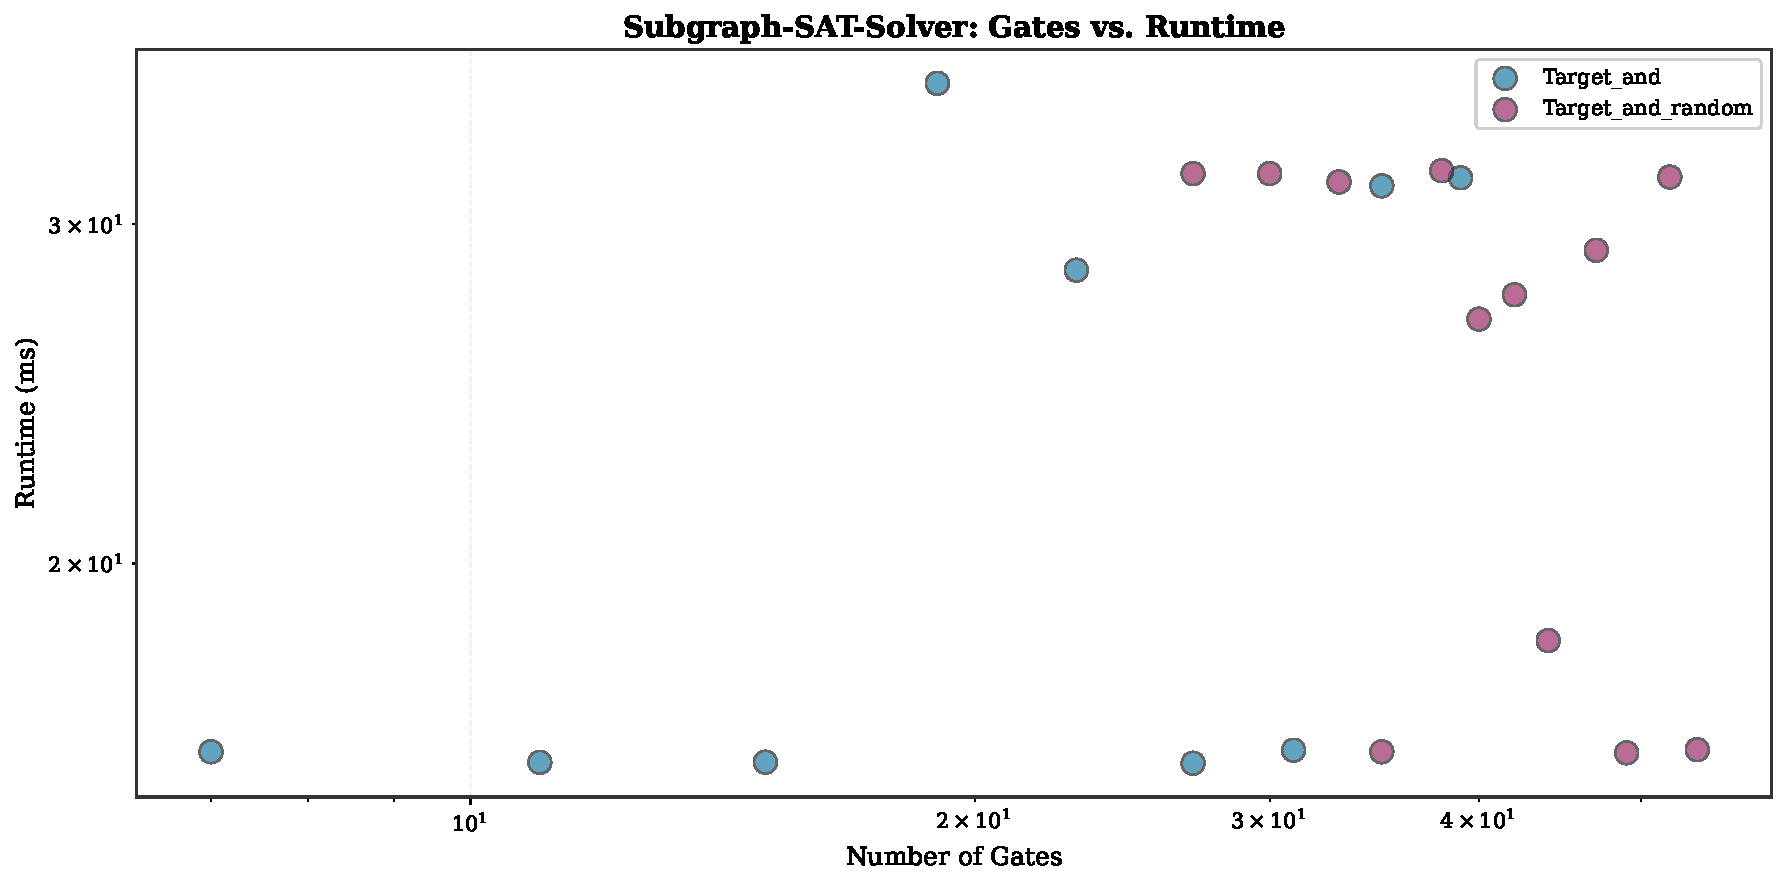
\includegraphics[width=\textwidth]{quick/plots/gates_vs_runtime.pdf}
	\caption{Quick}
\end{subfigure}\hfill
\begin{subfigure}[b]{0.48\textwidth}
	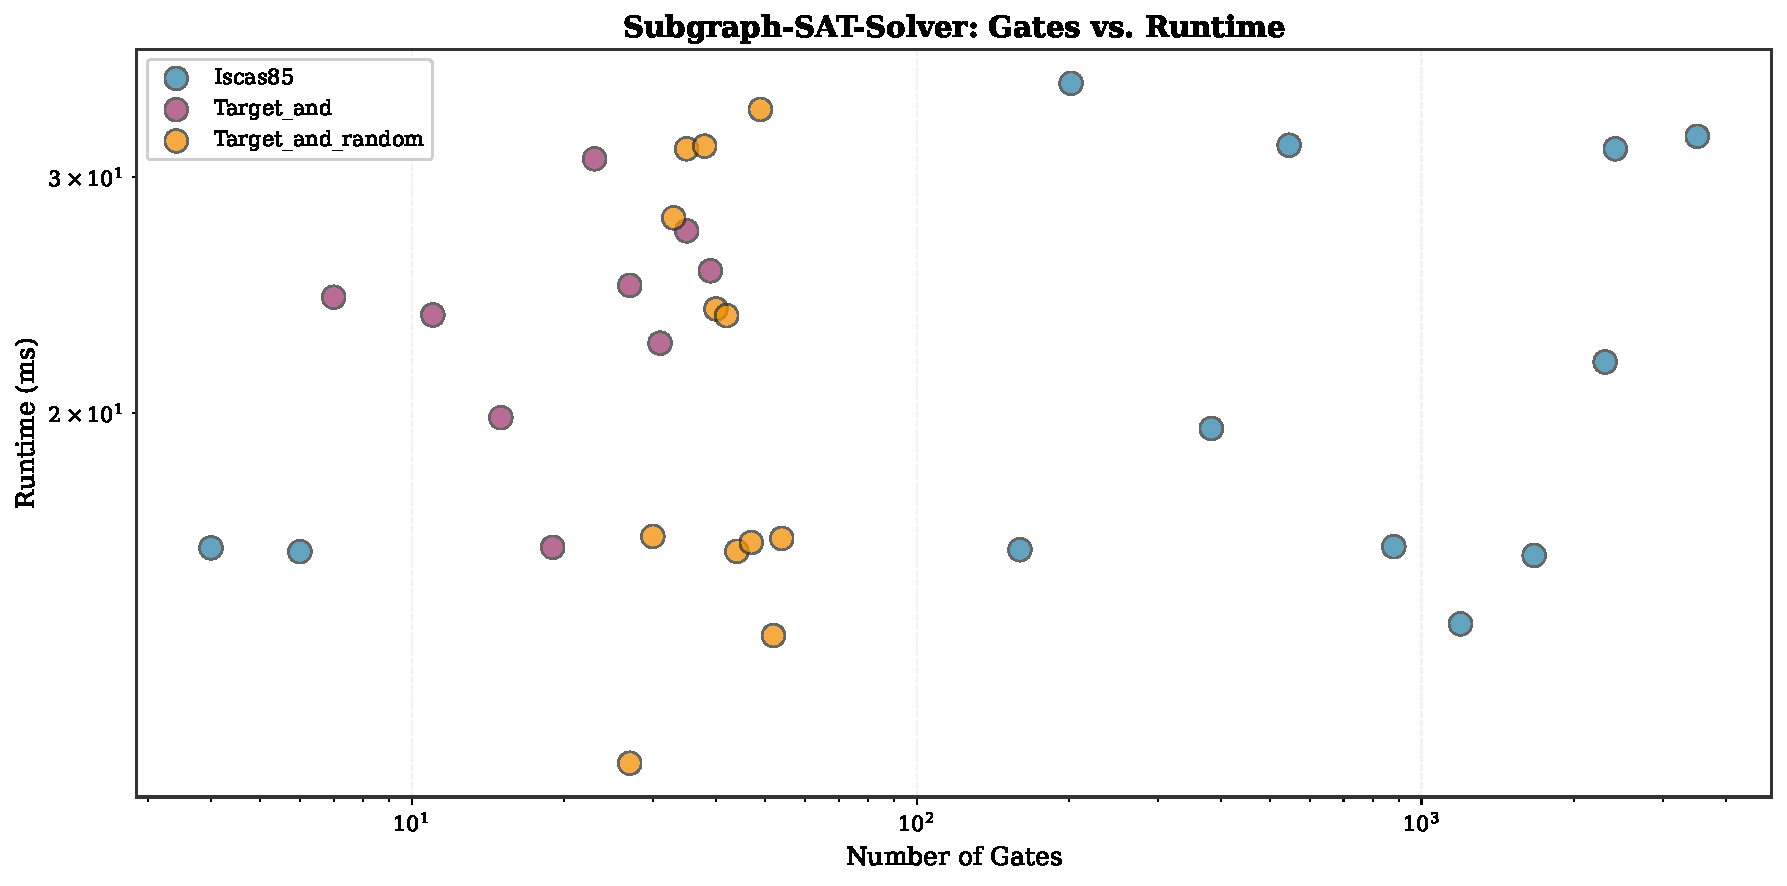
\includegraphics[width=\textwidth]{standard/plots/gates_vs_runtime.pdf}
	\caption{Standard}
\end{subfigure}

\vspace{0.5em}
\begin{subfigure}[b]{0.48\textwidth}
	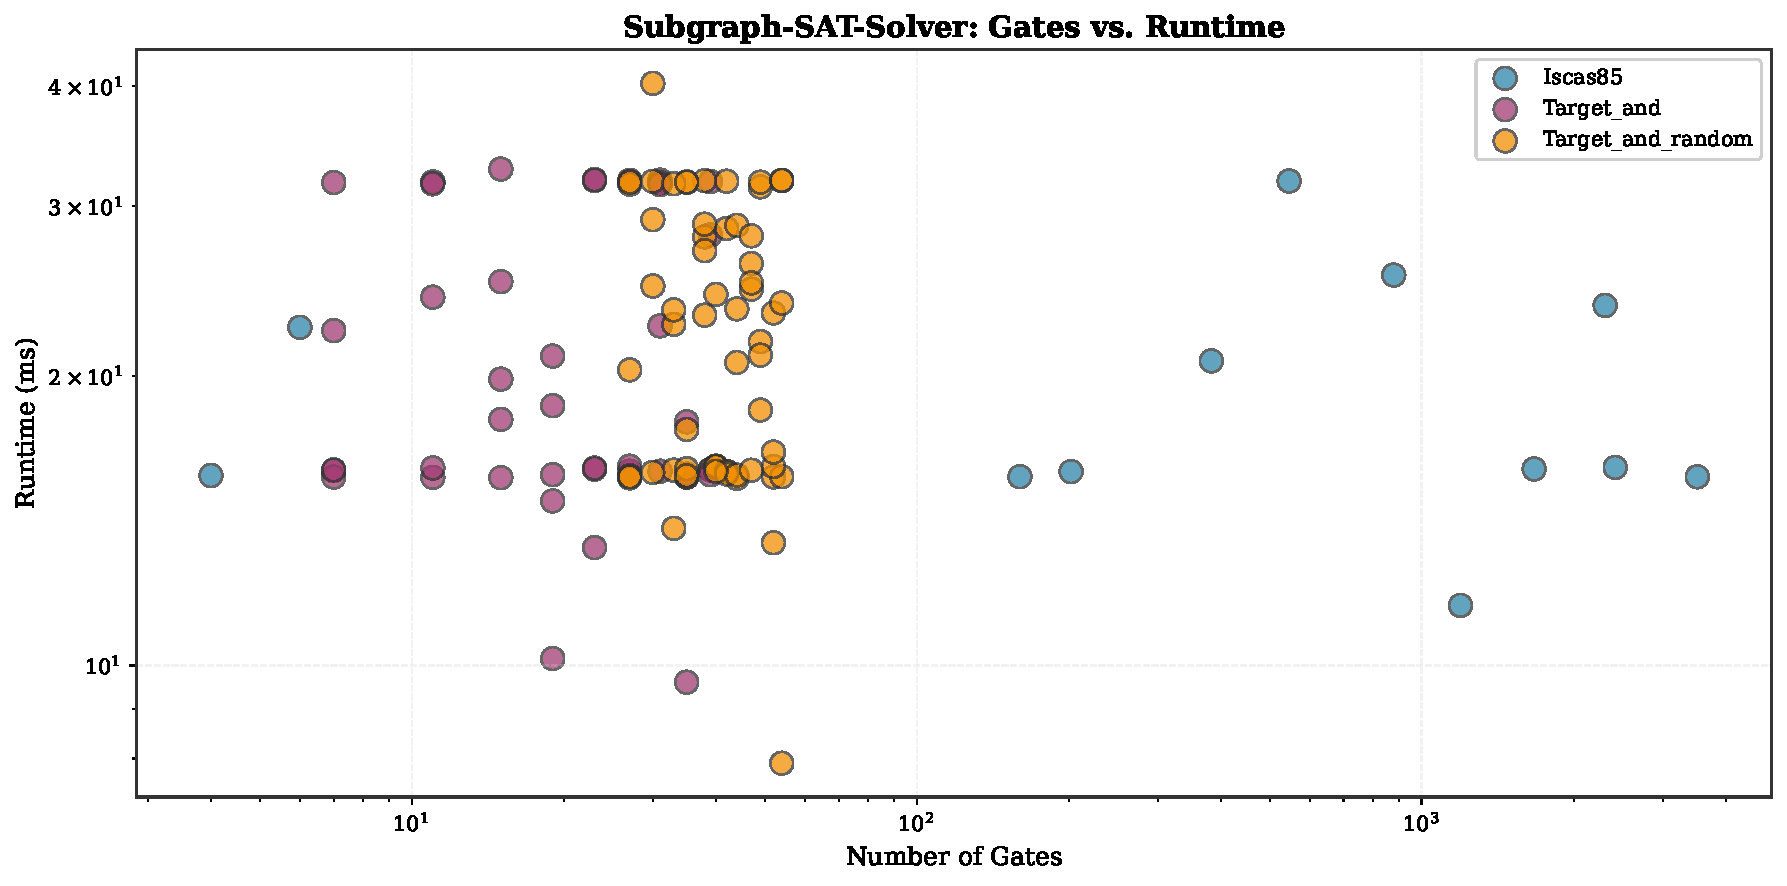
\includegraphics[width=\textwidth]{full/plots/gates_vs_runtime.pdf}
	\caption{Full}
\end{subfigure}\hfill
\begin{subfigure}[b]{0.48\textwidth}
	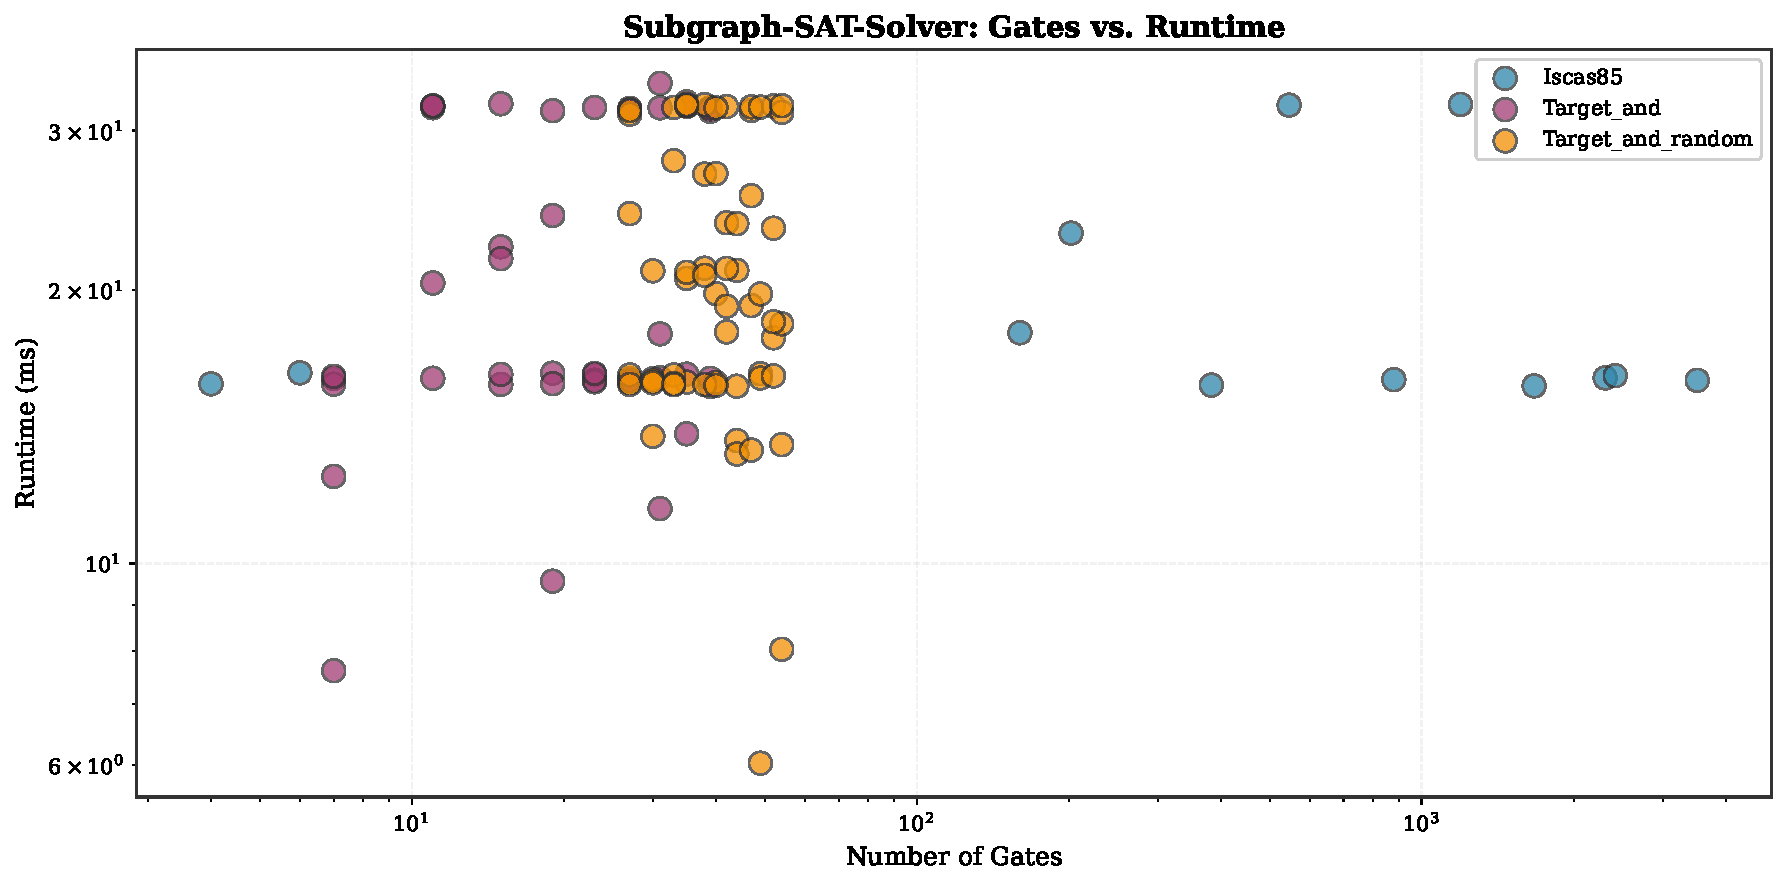
\includegraphics[width=\textwidth]{performance/plots/gates_vs_runtime.pdf}
	\caption{Performance}
\end{subfigure}
\caption{Gates gegen Laufzeit je Suite (vom Framework erzeugte Diagramme). Beide Achsen sind logarithmisch; Achsenbereiche und Farbzuordnung werden je Teilbild automatisch gewählt (in (a) blau: Target\_and, magenta: Target\_and\_random; in (b)--(d) blau: Iscas85, magenta: Target\_and, orange: Target\_and\_random).}
\label{fig:suiteplots}
\end{figure}

\paragraph{Gemeinsame Merkmale der vier Teilbilder.} Jedes Teilbild trägt den Titel \glqq Subgraph-SAT-Solver: Gates vs.\ Runtime\grqq{} und zeigt die Anzahl der Gates (Abszisse) gegen die Laufzeit in ms (Ordinate). Anders als in Abbildung~\ref{fig:gates} sind \emph{beide} Achsen logarithmisch; die Ordinate ist mit Beschriftungen wie $2 \times 10^{1}$ oder $3 \times 10^{1}$ versehen, sodass Abstände auf ihr nicht linear zu lesen sind (eine Verdopplung von $15{,}625$ auf $31{,}25$\,ms entspricht überall dem gleichen Abstand). Jeder Lauf ist ein großer, leicht transparenter Punkt ohne horizontale Verschiebung; Läufe mit identischer Gate-Anzahl und nahezu gleicher Laufzeit verdecken sich daher gegenseitig. Die Legende verwendet die Rohbezeichnungen des Frameworks. Zu beachten ist, dass die Farben je Teilbild vergeben werden und deshalb nicht überall demselben Typ entsprechen (siehe Bildunterschrift). Die Achsenbereiche sind ebenfalls je Teilbild automatisch gewählt, die vier Teilbilder sind also nicht unmittelbar maßstabsgleich.

\paragraph{(a) Quick.} Das Teilbild enthält $21$ Punkte: $9$ Target-AND- (blau) und $12$ Target-AND-Random-Läufe (magenta) zwischen $7$ und $54$ Gates. Es gibt keinen ISCAS-Lauf, daher endet die Abszisse bei etwa $54$ Gates. Die Laufzeiten reichen von $15{,}75$ bis $35{,}50$\,ms. Die Punkte ordnen sich in zwei Reihen an: acht Punkte bei etwa $15{,}8$ bis $16$\,ms am unteren Rand, sieben bei etwa $31{,}4$ bis $32$\,ms im oberen Bereich; zusammen sind das $15$ von $21$ Läufen ($71{,}4\,\%$) innerhalb von $\pm 1$\,ms um die beiden Zeittakte. Von den verbleibenden sechs Punkten liegen fünf dazwischen ($18{,}24$ bis $29{,}08$\,ms); der sechste ist der Höchstwert $35{,}50$\,ms bei $19$ Gates. Weil jede Instanz nur einmal läuft, gibt es keine senkrechten Stapel. Ein Anstieg zu größeren Gate-Zahlen ist nicht zu erkennen; der höchste Punkt gehört zu einem der kleineren Circuits.

\paragraph{(b) Standard.} Mit $33$ Läufen kommen erstmals die $12$ ISCAS-Circuits hinzu (blau), wodurch die Abszisse bis $3\,512$ Gates reicht. Die Laufzeiten liegen zwischen $10{,}97$ ($27$ Gates, Target-AND-Random) und $35{,}24$\,ms (c499 mit $202$ Gates). Die ISCAS-Punkte verteilen sich über den gesamten Wertebereich ohne Anstieg zu den großen Circuits: Der Median der ISCAS-Läufe beträgt $17{,}70$\,ms, der kleinste Wert $13{,}93$\,ms; am unteren Band stehen sowohl sehr kleine (c3, c17) als auch große Circuits. $16$ von $33$ Läufen ($48{,}5\,\%$) liegen innerhalb von $\pm 1$\,ms um die Zeittakte, der geringste Anteil aller vier Suites.

\paragraph{(c) Full.} Dieses Teilbild enthält $117$ Läufe, davon $12$ ISCAS-Läufe. Hier wird jeder synthetische Circuit fünfmal ausgeführt, die fünf Läufe haben dieselbe Gate-Anzahl und bilden senkrechte Stapel. Besonders dicht ist die Säule der Target-AND-Random-Circuits (orange) zwischen $27$ und $54$ Gates, in der sich zahlreiche Punkte überdecken; sichtbar sind deshalb mehr die beiden Bänder bei $16$ und $32$\,ms als die Einzelpunkte. Am oberen Rand steht bei $30$ Gates der Einzelwert $40{,}27$\,ms, am unteren Rand bei $54$ Gates der Einzelwert $7{,}91$\,ms; beide stammen von Target-AND-Random-Circuits ($d = 2$ bzw.\ $d = 12$). Mindestens die Hälfte der ISCAS-Läufe liegt bei höchstens $16{,}03$\,ms (Median), also am unteren Band. $69$ von $117$ Läufen ($59{,}0\,\%$) liegen nahe den Zeittakten.

\paragraph{(d) Performance.} Aufbau und Besetzung entsprechen (c). Die Ordinate beginnt tiefer (bei etwa $6$\,ms), weil hier der kleinste Wert der gesamten Studie liegt: $6{,}02$\,ms bei $49$ Gates (Target-AND-Random, $d = 10$). Daneben fallen weitere Werte unter $10$\,ms auf ($7{,}62$\,ms bei $7$ Gates, $8{,}04$\,ms bei $54$ Gates). Nach oben endet die Punktwolke bei $33{,}83$\,ms; es gibt also keinen Ausreißer wie in (c). Der Median der ISCAS-Läufe liegt bei $16{,}06$\,ms; mindestens die Hälfte der blauen Punkte steht damit am unteren Band. $73$ von $117$ Läufen ($62{,}4\,\%$) liegen nahe den Zeittakten, der höchste Anteil der vier Suites.

\paragraph{Vergleich der Teilbilder.} In allen vier Teilbildern zeigt sich dasselbe Muster aus zwei horizontalen Bändern bei etwa $15{,}6$ bis $16$\,ms und $31$ bis $32$\,ms, das unabhängig von Gate-Anzahl und Circuit-Typ auftritt. Mit wachsender Zahl der Läufe von (a) nach (c) und (d) wird dieses Muster deutlicher, weil mehr Punkte auf den Bändern liegen. Der Anteil der Läufe nahe den Zeittakten ($71{,}4$, $48{,}5$, $59{,}0$ und $62{,}4\,\%$) schwankt zwischen den Suites, folgt aber keiner Ordnung. Dieselbe Zeitauflösung ist demnach in allen Suites wirksam.

%=====================================================================
\begin{thebibliography}{99}

\bibitem{epp-subgraph}
S.~Epp. \emph{Der Subgraph Algorithmus}. Wissenschaftliche Arbeit, 2026. \url{https://github.com/naphez86/subgraph}.

\bibitem{epp2013}
S.~Epp. \emph{Learning M-DNF in Boolean Circuits}. Abschlussarbeit (Masterarbeit) im Masterstudiengang Informatik, Universität Paderborn, 2013.

\bibitem{brglez1985}
F.~Brglez, H.~Fujiwara. A neutral netlist of 10 combinational benchmark circuits and a target translator in Fortran. \emph{Proc.\ IEEE International Symposium on Circuits and Systems (ISCAS)}, 1985.

\bibitem{tseitin1968}
G.~S.~Tseitin. On the complexity of derivation in propositional calculus. \emph{Studies in Constructive Mathematics and Mathematical Logic, Part II}, 1968.

\bibitem{cook1971}
S.~A.~Cook. The complexity of theorem-proving procedures. \emph{Proc.\ 3rd Annual ACM Symposium on Theory of Computing (STOC)}, 1971.

\bibitem{karp1972}
R.~M.~Karp. Reducibility among combinatorial problems. In R.~E.~Miller and J.~W.~Thatcher, editors, \emph{Complexity of Computer Computations}, pages 85--103. Plenum Press, 1972.

\bibitem{levin1973}
L.~A.~Levin. Universal search problems. \emph{Problems of Information Transmission}, 9(3):265--266, 1973.

\bibitem{garey1979}
M.~R.~Garey and D.~S.~Johnson. \emph{Computers and Intractability: A Guide to the Theory of NP-Completeness}. W.~H.~Freeman, 1979.

\bibitem{papadimitriou1994}
C.~H.~Papadimitriou. \emph{Computational Complexity}. Addison-Wesley, 1994.

\bibitem{arora2009}
S.~Arora and B.~Barak. \emph{Computational Complexity: A Modern Approach}. Cambridge University Press, 2009.

\bibitem{sipser2012}
M.~Sipser. \emph{Introduction to the Theory of Computation}. 3rd edition, Cengage Learning, 2012.

\bibitem{ladner1975}
R.~E.~Ladner. On the structure of polynomial time reducibility. \emph{Journal of the ACM}, 22(1):155--171, 1975.

\bibitem{berman1977}
L.~Berman and J.~Hartmanis. On isomorphisms and density of NP and other complete sets. \emph{SIAM Journal on Computing}, 6(2):305--322, 1977.

\bibitem{cookreckhow1979}
S.~A.~Cook and R.~A.~Reckhow. The relative efficiency of propositional proof systems. \emph{Journal of Symbolic Logic}, 44(1):36--50, 1979.

\bibitem{davisputnam1960}
M.~Davis and H.~Putnam. A computing procedure for quantification theory. \emph{Journal of the ACM}, 7(3):201--215, 1960.

\bibitem{davislogemannloveland1962}
M.~Davis, G.~Logemann, and D.~Loveland. A machine program for theorem-proving. \emph{Communications of the ACM}, 5(7):394--397, 1962.

\bibitem{robinson1965}
J.~A.~Robinson. A machine-oriented logic based on the resolution principle. \emph{Journal of the ACM}, 12(1):23--41, 1965.

\bibitem{schaefer1978}
T.~J.~Schaefer. The complexity of satisfiability problems. In \emph{Proceedings of the 10th Annual ACM Symposium on Theory of Computing (STOC)}, pages 216--226, 1978.

\bibitem{monien1985}
B.~Monien and E.~Speckenmeyer. Solving satisfiability in less than $2^n$ steps. \emph{Discrete Applied Mathematics}, 10(3):287--295, 1985.

\bibitem schoning1999
U.~Sch\"oning. A probabilistic algorithm for $k$-SAT and constraint satisfaction problems. In \emph{Proceedings of the 40th Annual Symposium on Foundations of Computer Science (FOCS)}, pages 410--414, 1999.

\bibitem{impagliazzo2001}
R.~Impagliazzo and R.~Paturi. On the complexity of $k$-SAT. \emph{Journal of Computer and System Sciences}, 62(2):367--375, 2001.

\bibitem{paturi2005}
R.~Paturi, P.~Pudl\'ak, M.~E.~Saks, and F.~Zane. An improved exponential-time algorithm for $k$-SAT. \emph{Journal of the ACM}, 52(3):337--364, 2005.

\bibitem{grasp1999}
J.~P.~Marques-Silva and K.~A.~Sakallah. GRASP: A search algorithm for propositional satisfiability. \emph{IEEE Transactions on Computers}, 48(5):506--521, 1999.

\bibitem{chaff2001}
M.~W.~Moskewicz, C.~F.~Madigan, Y.~Zhao, L.~Zhang, and S.~Malik. Chaff: Engineering an efficient SAT solver. In \emph{Proceedings of the 38th Design Automation Conference (DAC)}, pages 530--535, 2001.

\bibitem{minisat2003}
N.~E\'en and N.~S\"orensson. An extensible SAT-solver. In E.~ Giunchiglia and A.~ Tacchella, editors, \emph{Theory and Applications of Satisfiability Testing (SAT 2003)}, Lecture Notes in Computer Science, volume 2919, pages 502--518. Springer, 2004.

\bibitem{plaisted1986}
D.~A.~Plaisted and S.~Greenbaum. A structure-preserving clause form translation. \emph{Journal of Symbolic Computation}, 2(3):293--304, 1986.

\bibitem{biere2009}
A.~Biere, M.~Heule, H.~van Maaren, and T.~ Walsh, editors. \emph{Handbook of Satisfiability}. Frontiers in Artificial Intelligence and Applications, volume 185. IOS Press, 2009.

\end{thebibliography}

\end{document}
